\chapter{Vectores.}

La Física es una ciencia que estudia cantidades físicas observables (medibles cuantitativamente) y las relaciones que pueden existir entre sus valores determinados experimentalmente. Algunas cantidades físicas requieren únicamente de la determinación de un solo número para su completa especificación. Temperatura, volumen, tiempo, longitud de recorrido, velocidad de la luz, frecuencia de una onda de sonido y carga eléctrica, son ejemplos de tales cantidades físicas, que son denominadas escalares. Por otra parte, hay cantidades físicas que requieren de dos o más números para su completa especificación. Para especificar un desplazamiento rectilíneo, por ejemplo, no es suficiente medir únicamente la magnitud del desplazamiento, sino que, para especificarlo en el espacio tridimensional, nos hacen falta dos cantidades más, con las que podremos determinar la dirección y sentido en que tiene lugar el desplazamiento. Cualquier cantidad física que, como el desplazamiento rectilíneo, requiera de una magnitud, una dirección y un sentido para su especificación, y que, además, pueda ser añadida a otra cantidad física similar, del mismo modo que son añadidos dos 
desplazamientos consecutivos para formar una sola cantidad física, también con una magnitud, una dirección y un sentido, recibe el nombre de cantidad vectorial tridimensional o simplemente vector tridimensional. En este capítulo familiarizaremos al lector con el lenguaje matemático y la manipulación matemática fundamental de los vectores tridimensionales. En uno de los últimos capítulos generalizaremos nuestros resultados para vectores de $n$ dimensiones, que son cantidades que requieren de $n$ números para su especificación. 
\par
Usaremos las letras negritas para señalar los vectores y distinguirlos de los escalares, que estarán indicados por letras cursivas. Asi, $\vb{A}$ representa un vector, mientras que su magnitud, siendo un número puro o escalar, será representada por $A$. En ocasiones, también utilizaremos $\abs{A}$ para representar la magnitud $A$ del vector $\vb{A}$.

\section{Representación geométrica de un vector.} 

Gráficamente podemos representar la dirección, sentido y magnitud de un vector por un segmento de recta dirigido, o sea, con una flecha trazada paralelamente al vector y apuntando en el sentido de éste. La longitud de la flecha será dibujada a escala, de manera que esta longitud pueda representar la magnitud del vector. En la figura (\ref{fig:figura_01_01}), por ejemplo, representamos gráficamente un vector $\vb{A}$, paralelo al plano $x y$ y que forma un ángulo $\phi$ con una recta paralela al eje $x$. Si el vector $\vb{A}$ tiene una magnitud de cinco unidades, entonces, la longitud de la flecha que lo representa se dibujaría igual a cinco veces la longitud escogida para representar al vector de magnitud unidad. 
\begin{figure}[H]
    \centering
    \begin{tikzpicture}
        \draw (0, 0) -- (5, 0) node[below, pos=1.05] {$x$};
        \draw (0, 0) -- (0, 4) node[left, pos=1.05] {$y$};
        \draw [-stealth, thick] (1, 1) -- (3, 3) node[above, midway] {$\vb{A}$};
        \draw [dashed] (1, 1) -- (3, 1);
        \draw (1.5, 1) arc(0:30:0.75) node[right] {$\phi$};
    \end{tikzpicture}
    \caption{Representación gráfica de un vector $\vb{A}$ en el plano $x y$.}
    \label{fig:figura_01_01}
\end{figure}
De la representación de la magnitud de un vector por la longitud de una flecha deducimos que la multiplicación de un vector $\vb{A}$ por un escalar $c$ (positivo) da como producto un vector paralelo a $\vb{A}$, que tiene una magnitud igual a $c$ veces la magnitud de $\vb{A}$:
\begin{align}
    \abs{c \, \vb{A}} = c \, A
    \label{eq:ecuacion_01_01}
\end{align} 
De esto, resulta que podríamos expresar cualquier vector como el producto de un escalar por un vector de magnitud uno, llamado vector unidad. Está claro que si $\vb{e}_{A}$ es el vector unidad en la dirección y sentido de $\vb{A}$, el vector $A \, \vb{e}_{A}$ es un vector en la dirección y sentido de $\vb{A}$ que tiene una magnitud $A$. 
\par
Se dice que dos vectores $\vb{A}$ y $\vb{B}$ son iguales si ambos tienen las mismas magnitud y dirección y el mismo sentido. Por lo tanto, podemos escribir:
\begin{align}
    \vb{B} = A \, \vb{e}_{A}
    \label{eq:ecuacion_01_02} 
\end{align}
El vector nulo $\vb{0}$ se define como un vector de magnitud igual a cero y, por lo tanto, no tiene dirección ni sentido.

\section{Suma y resta de vectores.}

La suma de dos vectores $\vb{A}$ y $\vb{B}$ está representada gráficamente en la figura (\ref{fig:figura_01_02}). Para sumar gráficamente dos vectores $\vb{A}$ y $\vb{B}$, dibujamos la flecha que representa al vector $\vb{A}$, y desde su punta trazaremos la flecha que representa al vector $\vb{B}$. El vector $\vb{C}$, que es la suma de los dos vectores, está entonces representado por la flecha dibujada desde la cola de la flecha de $\vb{A}$, hasta la punta de la de $\vb{B}$. Esta regla para la suma de vectores se llama \emph{ley de adición del paralelogramo}.
\begin{figure}[H]
    \centering
    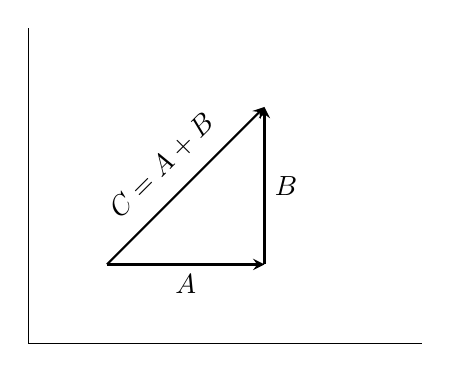
\begin{tikzpicture}
        \draw (0, 0) -- (5, 0);
        \draw (0, 0) -- (0, 4);
        \draw [-stealth, thick] (1, 1) -- (3, 3);
        \node[rotate=45] at (1.7, 2.25) {$\vb{C} = \vb{A} + \vb{B}$};
        \draw [-stealth, thick] (1, 1) -- (3, 1) node [below, midway] {$\vb{A}$};
        \draw [-stealth, thick] (3, 1) -- (3, 3) node [right, midway] {$\vb{B}$};
    \end{tikzpicture}
    \caption{Representación gráfica de la suma de dos vectores.}
    \label{fig:figura_01_02}
\end{figure}
En la figura (\ref{fig:figura_01_03}) podemos ver que la suma de vectores es conmutativa:
\begin{align*}
    \vb{A} + \vb{B} = \vb{B} + \vb{A}
\end{align*}
\begin{figure}[H]
    \centering
    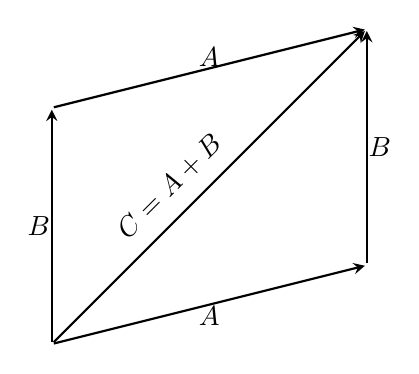
\begin{tikzpicture}[inner sep=0pt]
        \node at (0, 0) (A) {};
        \node at (4, 1) (B) {};
        \node at (4, 4) (C) {};
        \node at (0, 3) (D) {};
        \draw [-stealth, thick] (A) -- (B) node [below=0.25, midway] {$\vb{A}$};
        \draw [-stealth, thick] (B) -- (C) node [right=0.25, midway] {$\vb{B}$};
        \draw [-stealth, thick] (A) -- (C);
        \node at (1.5, 2) [rotate=45] {$\vb{C} = \vb{A} + \vb{B}$};
        \draw [-stealth, thick] (A) -- (D) node [left=0.25, midway] {$\vb{B}$};
        \draw [-stealth, thick] (D) -- (C) node [above=0.25, midway] {$\vb{A}$};
    \end{tikzpicture}
    \caption{Naturaleza conmutativa de la suma vectorial: $\vb{A} + \vb{B} = \vb{B} + \vb{A}$.}
    \label{fig:figura_01_03}
\end{figure}
La suma de vectores es también asociativa, ver la figura (\ref{fig:figura_01_04}):
\begin{align*}
    \vb{A} + \left( \vb{B} + \vb{C} \right) = \left( \vb{A} + \vb{B} \right) + \vb{C}
\end{align*}
\begin{figure}[H]
    \centering
    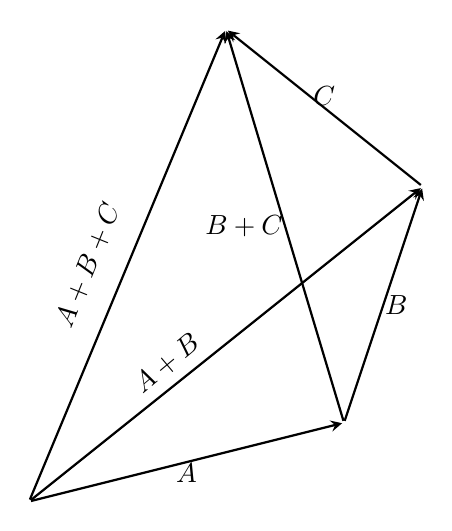
\begin{tikzpicture}[inner sep=0pt]
        \node at (0, 0) (A) {};
        \node at (4, 1) (B) {};
        \node at (5, 4) (C) {};
        \node at (2.5, 6) (D) {};
        \draw [-stealth, thick] (A) -- (B) node [below=0.25, midway] {$\vb{A}$};
        \draw [-stealth, thick] (B) -- (C) node [right=0.25, midway] {$\vb{B}$};
        \draw [-stealth, thick] (A) -- (C);
        \node at (1.75, 1.75) [rotate=40] {$\vb{A} + \vb{B}$};
        \draw [-stealth, thick] (C) -- (D) node [above=0.25, midway] {$\vb{C}$};
        % \draw [-stealth, thick] (A) -- (D) node [left=0.25, midway] {$\vb{B}$};
        % \draw [-stealth, thick] (D) -- (C) node [above=0.25, midway] {$\vb{A}$};
        \draw [-stealth, thick] (B) -- (D) node [left=0.23, pos=0.5] {$\vb{B} + \vb{C}$};
        \draw [-stealth, thick] (A) -- (D);
        \node at (0.75, 3) [rotate=68] {$\vb{A} + \vb{B} + \vb{C}$};
    \end{tikzpicture}
    \caption{Naturaleza asociativa de la suma vectorial : $\vb{A} + \left( \vb{B} + \vb{C} \right) = \left( \vb{A} + \vb{B} \right) + \vb{C}$.}
    \label{fig:figura_01_04}
\end{figure}
Si la suma de dos vectores $\vb{A}$ y $\vb{B}$ es igual a un vector dé magnitud cero:
\begin{align}
    \vb{A} + \vb{B} = \vb{0}
    \label{eq:ecuacion_01_03}
\end{align}
entonces, los dos vectores $\vb{A}$ y $\vb{B}$, obviamente, deben tener iguales magnitud y dirección y sentidos opuestos. Asi, la ecuación (\ref{eq:ecuacion_01_03}) queda :
\begin{align}
    \vb{B} = - \vb{A}
    \label{ec:ecuacion_01_04}
\end{align}
que nos dice que $- \vb{A}$ es un vector que tiene la misma magnitud (y dirección) del vector $\vb{A}$, pero apunta en un sentido opuesto al de éste. 
\par
Esto nos permite definir la resta del vector $\vb{B}$ al vector $\vb{A}$, como la suma del vector $\vb{A}$ y el vector $\left( - \vb{B} \right)$: 
\begin{align}
    \vb{A} - \vb{B} = \vb{A} + \left( - \vb{B} \right)
    \label{eq:ecuacion_01_05}
\end{align}

\section{Representación algebraica de un vector.}

Cualquier vector $\vb{A}$, como demostraremos, puede ser representado algebraicamente, especificando sus proyecciones sobre un sistema de ejes 
coordenados o de vectores base. Los tres vectores base de un sistema de coordenadas tridimensional deben ser independientes linealmente; por 
tanto, deben satisfacer el requisito de no ser coplanares. La elección más simple, aunque no queremos decir que sea la única, para tal sistema de vectores base no coplanares, es un sistema de vectores unidad perpendiculares entre sí. 
\par
En un sistema de coordenadas cartesianas se escogerán como los tres vectores base los vectores unidad tomados y dirigidos respectivamente a lo 
largo de los ejes $x$, $y$ y $z$ positivos. Los vectores unidad sobre los ejes coordenados $x$, $y$ y $z$ positivos se designarán, respectivamente, por los símbolos $\vb{i}$, $\vb{j}$ y $\vb{k}$ (figura \ref{fig:figura_01_05}). A veces, también encontraremos notacionalmente conveniente designarlos por los símbolos $\vb{e}_{1}, \vb{e}_{2}$ y $\vb{e}_{3}$.
\begin{figure}[H]
    \centering
    \tdplotsetmaincoords{70}{110}
    \begin{tikzpicture}[tdplot_main_coords, scale=2]
        \draw[thick] (0, 0, 0) -- (2, 0, 0) node[anchor=north east] {$x$};
        \draw[thick] (0, 0, 0) -- (0, 1.25, 0) node[anchor=north west] {$y$};
        \draw[thick] (0, 0, 0) -- (0, 0, 1) node[anchor=south] {$z$};
        \draw[line width=0.5mm, -stealth] (0, 0, 0) -- (1, 0, 0) node[above, pos=0.9] {$\vb{i}$};
        \draw[line width=0.5mm, -stealth] (0, 0, 0) -- (0, 0.5, 0) node[above, pos=0.9] {$\vb{j}$};
        \draw[line width=0.5mm, -stealth] (0, 0, 0) -- (0, 0, 0.5) node[right, pos=0.9] {$\vb{k}$};
    \end{tikzpicture}
    \caption{Vectores base unitarios cartesianos.}
    \label{fig:figura_01_05}
\end{figure}
La proyección de un vector $\vb{A}$ sobre otro $\vb{B}$ está representada gráficamente por la longitud del segmento rectilíneo comprendido entre la intersección de una recta paralela a $\vb{B}$ con las perpendiculares a la dirección de $\vb{B}$ desde la cola y la punta de la flecha que representa a $\vb{A}$ (figura \ref{fig:figura_01_06}).
\begin{figure}[H]
    \centering
    \begin{tikzpicture}
        \draw (-0.5, -0.5) -- (6, -0.5);
        \draw (-0.5, -0.5) -- (-0.5, 4);
        \draw [-stealth, thick] (1, 1) -- (4, 3) node[above=0.25, midway] {$\vb{A}$};
        \draw [dashed] (4, 3) -- (4, 1);
        \draw (1, 1) -- (5, 1);
        \draw (1.5, 1) arc(0:30:0.5) node[right] {$\phi$};
        \draw (1, 1) -- (1, 0.6);
        \draw (4, 1) -- (4, 0.6);
        \draw [-stealth] (1.3, 0.7) -- (1, 0.7);
        \draw [-stealth] (3.7, 0.7) -- (4, 0.7);
        \node at (2.5, 0.7) {\small{$A_{B} = A \cos \phi$}};
        \draw [-stealth, thick] (2.5, 0.15) -- (5.5, 0.15) node[below, midway] {$\vb{B}$};
    \end{tikzpicture}
    \caption{Proyección del vector $\vb{A}$ sobre el vector $\vb{B}$.}
    \label{fig:figura_01_06}
\end{figure}
Si la proyección sobre $\vb{B}$ de la punta de la flecha que representa a $\vb{A}$, se halla en el sentido de $\vb{B}$ con respecto a la proyección de la cola de dicha flecha sobre $\vb{B}$, entonces, la proyección será considerada positiva. Si está dirigida en sentido opuesto, será considerada negativa. En relación con el más pequeño de los dos ángulos, el ángulo $\phi$, que forma la flecha que representa al vector $\vb{A}$ con una flecha trazada en la dirección y sentido de $\vb{B}$, a partir del pie de la flecha de $\vb{A}$, la proyección de $\vb{A}$ sobre $\vb{B}$, también llamada componente $\vb{B}$ de $\vb{A}$ y designada por $A_{B}$ , está dada por la fórmula:
\begin{align}
    A_{B} = A \cos \phi
    \label{eq:ecuacion_01_06}
\end{align}
El ángulo $\phi$ será mencionado como el ángulo entre los vectores $\vb{A}$ y $\vb{B}$. 
\par
De acuerdo con la regla por la que indicamos que una proyección es positiva o negativa, encontramos que $A_{B}$ es positiva para:
\begin{align*}
    0 < \phi < \dfrac{\pi}{2}
\end{align*}
y negativa para:
\begin{align*}
    \dfrac{\pi}{2} < \phi < \pi
\end{align*}
De la ley de la suma se desprende que el vector $\vb{A}$ se puede expresar por la suma de tres vectores $A_{x} \, \vb{i}, A_{y} \, \vb{j}$ y $A_{z} \, \vb{k}$. Esto es:
\begin{align}
    \vb{A} = A_{x} \, \vb{i} + A_{y} \, \vb{j} + A_{z} \, \vb{k}
    \label{eq:ecuacion_01_07}
\end{align}
donde $A_{x}, A_{y}$ y $A_{z}$ son las componentes de $\vb{A}$ sobre los ejes $x, y, z$ positivos. Por ejemplo, considérese un vector $\vb{A}$ que esté en el plano $x y$ $(A_{z} = 0)$. En este caso, siempre podremos imaginar al vector $\vb{A}$ situado sobre la hipotenusa de un triángulo rectángulo cuyos catetos sean paralelos a los ejes $x$ y $y$ positivos. De la figura (\ref{fig:figura_01_07}) resulta evidente que:
\begin{align}
    A_{x} &= A \cos \phi \label{eq:ecuacion_01_08} \\
    A_{y} &= A \sin \phi \label{eq:ecuacion_01_09}
\end{align}
y que la relación:
\begin{align}
    A^{2} &= A_{x}^{2} + A_{y}^{2} \label{eq:ecuacion_01_10} \\
    \vb{A} &= A_{x} \, \vb{i} + A_{y} \, \vb{j} \label{eq:ecuacion_01_11}
\end{align}
es correcta.
\begin{figure}[H]
    \centering
    \begin{tikzpicture}
        \pic at (0, 0) {ejesxy};
        \draw [-stealth, thick] (0, 0) -- (3, 3) node[above=0.25, midway] {$\vb{A}$};
        \draw [-stealth, thick] (0, 0) -- (3, 0) node[below, midway] {$A_{x} \, \vb{i}$};
        \draw [-stealth, thick] (3, 0) -- (3, 3) node[right, midway] {$A_{y} \, \vb{j}$};
        \draw (0.5, 0) arc(0:45:0.5) node[right] {$\phi$};
    \end{tikzpicture}
    \caption{Prueba gráfica de $\vb{A} = A_{x} \, \vb{i} + A_{y} \, \vb{j}$ para un vector paralelo al plano $x y$.}
    \label{fig:figura_01_07}
\end{figure}
La extensión a vectores tridimensionales se muestra en la figura (\ref{fig:figura_01_08}). En relación con el ángulo $\theta$ que forma el vector $\vb{A}$ con el eje $z$ positivo y el ángulo $\phi$ que forma la proyección de $\vb{A}$ sobre el plano $x y$ con el eje $x$ positivo, resulta que:
\begin{align}
    A_{x} &= A \sin \theta \cos \phi \label{eq:ecuacion_01_12} \\[0.5em]
    A_{y} &= A \sin \theta \sin \phi \label{eq:ecuacion_01_13} \\[0.5em]
    A_{z} &= A \cos \theta \label{eq:ecuacion_01_14} \\[0.5em]
    A^{2} &= A_{x}^{2} + A_{y}^{2} + A_{z}^{2} \label{eq:ecuacion_01_15}
\end{align}
y que realmente:
\begin{align*}
    \vb{A} &= A_{x} \, \vb{i} + A_{y} \, \vb{j} + A_{z} \, \vb{k}
\end{align*}
\begin{figure}[H]
    \centering
    \tdplotsetmaincoords{60}{120}
\begin{tikzpicture}
	[scale=3,
		tdplot_main_coords,
		axis/.style={-stealth, black, thick},
		vector/.style={-stealth, black, thick},
		vector guide/.style={blue, thick},
		angle/.style={red,thick}]

	%standard tikz coordinate definition using x, y, z coords
	\coordinate (O) at (0, 0, 0);
	
	%tikz-3dplot coordinate definition using r, theta, phi coords
	\tdplotsetcoord{P}{1.5}{55}{60}
	
	%draw axes
	\draw[axis] (0, 0, 0) -- (1.5, 0, 0) node [anchor=north east] {$x$};
	\draw[axis] (0, 0, 0) -- (0, 1, 0) node [anchor=north west] {$y$};
	\draw[axis] (0, 0, 0) -- (0, 0, 1) node [anchor=south] {$z$};
	
	%draw a vector from O to P
	\draw[vector] (O) -- (P) node [above, pos=0.7] {$\vb{A}$};
	
	%draw guide lines to components
	\draw[vector guide] (O) -- (Pxy);
	\draw[vector guide, -stealth] (Pxy) -- (P) node [right, pos=0.6] {$A_{z} \, \vb{k}$};


    \draw [-stealth, vector guide] (O) -- (Px) node [left, pos=0.5] {$A_{x} \, \vb{i}$};
    \draw [-stealth, vector guide] (Px) -- (Pxy) node [below, pos=0.75] {$A_{y} \, \vb{j}$};
    \node at (1, 0.35, 0) [blue, below] {$A_{x} \, \vb{i} + A_{y} \, \vb{j}$};
    \draw [blue, thick, -stealth] (1, 0.35, 0) -- (0.4, 0.65, 0);

	%draw an arc illustrating the angle defining the orientation
	\tdplotdrawarc[angle]{(O)}{.25}{0}{60}{anchor=north}{$\phi$}

	%define the rotated coordinate frame to lie in the "theta plane"
	\tdplotsetthetaplanecoords{55}
	
	\tdplotdrawarc[tdplot_rotated_coords,angle]{(O)}{.35}{0}{55}
          {anchor=south west}{$\theta$}

    \end{tikzpicture}
    \caption{Prueba gráfica de $\vb{A} = A_{x} \, \vb{i} + A_{y} \, \vb{j} + A_{z} \, \vb{k}$}
    \label{fig:figura_01_08}
\end{figure}
De la definición de igualdad de dos vectores resultará evidente que la de sus componentes $x, y, z$ es una condición necesaria y suficiente para que sean iguales. También sera claro que las componentes $x, y, z$ de la suma de dos o mas vectores son iguales a las sumas de las respectivas componentes de los vectores. Esto es, si el vector $\vb{C}$ es la suma de los vectores $\vb{A}$ y $\vb{B}$: 
\begin{align}
    \vb{C} = \vb{A} + \vb{B}
    \label{eq:ecuacion_01_16}
\end{align}
entonces:
\begin{align}
    C_{x} = A_{x} + B_{x}, \hspace{0.75cm} C_{y} = A_{y} + B_{y}, \hspace{0.75cm} C_{z} = A_{z} + B_{z} \label{eq:ecuacion_01_17}
\end{align}
de donde podemos obtener:
\begin{align}
    C^{2} = C_{x}^{2} + C_{y}^{2} + C_{z}^{2} &= A^{2} + B^{2} + 2 \left( A_{x} B_{x} + A_{y} B_{y} + A_{z} B_{z} \right) \nonumber \\[0.5em]
    &= A^{2} + B^{2} + 2 \, A \, B \, \cos \phi \label{eq:ecuacion_01_18}
\end{align}
La ultima expresión es la ley de los cosenos. Observaremos que el signo más frente al ultimo término del segundo miembro de la ecuación (\ref{eq:ecuacion_01_18}) se debe a que el ángulo entre los vectores $\vb{A}$ y $\vb{B}$ es el exterior del triángulo formado por estos vectores, ver la figura (\ref{fig:figura_01_09}). 
\begin{figure}[H]
    \centering
    \begin{tikzpicture}[inner sep=0pt]
        \node at (1, 0.5) (A) {};
        \node at (4, 1.5) (B) {};
        \node at (5, 4) (C) {};

        \pic at (0, 0) {ejesxy};

        \draw [-stealth, thick] (A) -- (B) node [below, midway] {$\vb{A}$};
        \draw [-stealth, thick] (B) -- (C) node [right=0.2, pos=0.7] {$\vb{B}$};
        \draw [-stealth, thick] (A) -- (C) node [above=0.2, midway] {$\vb{C}$};
        \draw (B) -- (5.5, 2);
        \draw (4.5, 1.7) arc(0:30:1.3) node[right=0.1, pos=0.5] {$\phi$};
    \end{tikzpicture}
    \caption{Ley de los cosenos $C^{2} = A^{2} + B^{2} + 2 \, A \, B \, \cos \phi$.}
    \label{fig:figura_01_09}
\end{figure}
La elección de la orientación del sistema de coordenadas $(x, y, z)$ es, por supuesto, arbitraria. Por lo tanto, dos vectores iguales tienen componentes iguales en cualquier dirección, y la componente en cualquier dirección de la suma de dos o más vectores es igual a la suma de las componentes de estos vectores en dicha dirección:
\begin{align}
    C_{D} = A_{D} + B_{D}
    \label{eq:ecuacion_01_19}
\end{align}

\section{Multiplicación vectorial.}

Dados los dos vectores $\vb{A}$ y $\vb{B}$, existen dos productos de estos vectores para los que encontraremos uso inmediato. El primer producto es el llamado \emph{producto escalar}, ya que nos da una cantidad escalar. Hemos hallado ya este producto en la ecuación (\ref{eq:ecuacion_01_18}). Se designa por $\vb{A} \cdot \vb{B}$, y está definido por la ecuación:
\begin{align}
    \vb{A} \cdot \vb{B} = A \, B \, \cos \phi
    \label{eq:ecuacion_01_20}
\end{align}
donde $\phi$ es el ángulo que forman los vectores $\vb{A}$ y $\vb{B}$. Como hemos visto, esta expresión aparece en la ley de los cosenos, de la que obtenemos la relación (fig. \ref{fig:figura_01_09}):
\begin{align}
    \vb{A} \cdot \vb{B} = \dfrac{C^{2} - A^{2} - B^{2}}{2} = A_{x} \, B_{x} + A_{y} \, B_{y} + A_{z} \, B_{z}
    \label{eq:ecuacion_01_21}
\end{align}
De su definición, el producto escalar es, obviamente, conmutativo:
\begin{align*}
    \vb{A} \cdot \vb{B} = \vb{B} \cdot \vb{A}
\end{align*}
Como la proyección de la suma de los vectores $\vb{A}$ y $\vb{B}$ sobre un vector $\vb{C}$ es igual a la suma de la proyección de $\vb{A}$ sobre $\vb{C}$ más la de $\vb{B}$ sobre $\vb{C}$, se encuentra que el producto escalar satisface la ley distributiva:
\begin{align*}
\left( \vb{A} + \vb{B} \right) \cdot \vb{C} = \vb{A} \cdot \vb{C} + \vb{B} \cdot \vb{C}
\end{align*}
El otro producto que necesitaremos es el producto vectorial de los dos vectores $\vb{A}$ y $\vb{B}$, indicado por $\vb{A} \cp \vb{B}$. Más adelante encontraremos este producto en la forma:
\begin{align}
\begin{aligned}[b]
\vb{A} \cp \vb{B} &= \mdet{
    \vb{i} & \vb{j} & \vb{k} \\
    A_{x} & A_{y} & A_{z} \\
    B_{x} & B_{y} & B_{z} } = \\[0.5em]
    &= \left( A_{y} B_{z} - A_{z} B_{y} \right) \vb{i} + \left( A_{z} B_{x} - A_{x} B_{z} \right) \vb{j} + \left( A_{x} B_{y} - A_{y} B_{x} \right) \vb{k}
\end{aligned}
\label{eq:ecuacion_01_22}
\end{align}
que utilizaremos como su definición.
\par
Sólo hace falta una simple manipulación algebraica para demostrar que:
\begin{align*}
\abs{\vb{A} \cp \vb{B}}^{2} = A^{2} B^{2} - \left( \vb{A} \cdot \vb{B} \right)^{2} =  A^{2} \, B^{2} \, \sin^{2} \phi
\end{align*}
o sea, que la magnitud del producto vectorial de los vectores $\vb{A}$ y $\vb{B}$ es:
\begin{align}
    \abs{\vb{A} \cp \vb{B}} = A \, B \, \sin \phi
    \label{eq:ecuacion_01_23}
\end{align}
donde $\phi$ es el ángulo entre los vectores $\vb{A}$ y $\vb{B}$. 
\par
El producto escalar de $\vb{A} \cp \vb{B}$ por uno cualquiera de los dos, $\vb{A}$ o $\vb{B}$, es cero. Por lo tanto, el producto vectorial $\vb{A} \cp \vb{B}$ forma un ángulo de $\ang{90}$ con cualquiera de los vectores $\vb{A}$ o $\vb{B}$ y es, por consiguiente, 
perpendicular al plano de dichos vectores, así como a cualquier plano paralelo a éste. Para una determinación más completa del producto vectorial necesitamos una especificación más precisa del sentido de $\vb{A} \cp \vb{B}$ a lo largo de la perpendicular al plano de $\vb{A}$ y $\vb{B}$, pues hay dos sentidos en la dirección de ésta. Para hallar cuál de estos dos es, hagamos que coincida el plano de $\vb{A}$ y $\vb{B}$ con el $x y$ y con el eje $x$ positivo situado sobre el vector $\vb{A}$ y en su mismo sentido. Con esta elección de los ejes coordenados, el producto vectorial está dado por:
\begin{align*}
\vb{A} \cp \vb{B} &= \mdet{
    \vb{i} & \vb{j} & \vb{k} \\
    A_{x} & 0 & 0 \\
    B_{x} & B_{y} & 0 } = A_{x} B_{y} \vb{k}
\end{align*}
Así, para $B_{y}$ positiva el producto vectorial de $\vb{A}$ y $\vb{B}$ está sobre el sentido positivo de $\vb{k}$, mientras que para una $B_{y}$ negativa está sobre el sentido negativo de $\vb{k}$. En este curso nos limitaremos a usar sistemas de coordenadas cartesianas de sentido a la derecha, para las cuales podemos establecer:
\begin{align}
    \vb{A} \cp \vb{B} = A \,B \sin \phi \, \vb{n}
    \label{eq:ecuacion_01_24}
\end{align}
donde $\vb{n}$ es un vector unitario perpendicular al plano de $\vb{A}$ y $\vb{B}$, en el sentido del avance de un tomillo de rosca a la derecha que es girado alrededor de un eje perpendicular al plano de $\vb{A}$ y $\vb{B}$, en el sentido que llevaría $\vb{A}$ sobre $\vb{B}$ al girarlo el más pequeño de los dos ángulos que forman los dos vectores (ver la fig. \ref{fig:figura_01_10}).
\begin{figure}[H]
    \centering
    \includegraphics[scale=1]{Imagenes/producto_vectorial_01.pdf}
    \caption{Definición de un producto vectorial en un sistema de coordenadas derecho.}
    \label{fig:figura_01_10}
\end{figure}
De la ecuación (\ref{eq:ecuacion_01_22}) se deduce que el producto vectorial no es conmutativo, sino que:
\begin{align}
    \vb{A} \cp \vb{B} = - \vb{B} \cp \vb{A}
    \label{eq:ecuacion_01_25}
\end{align} 
Sin embargo, la ley distributiva es válida:
\begin{align}
    \vb{A} \cp \left( \vb{B} + \vb{C} \right) = \vb{A} \cp \vb{B} + \vb{A} \cp \vb{C}
    \label{eq:ecuacion_01_26}   
\end{align}
Esto se demuestra fácilmente usando el determinante que nos sirvió para definir el producto vectorial (ec. \ref{eq:ecuacion_01_22}). 
\par
El producto escalar del vector $\vb{A}$ por el producto vectorial de los vectores $\vb{B}$ y $\vb{C}$ se llama triple producto escalar. En relación con las componentes cartesianas de estos vectores, el triple producto escalar está dado por:
\begin{align}
    \vb{A} \cdot \left( \vb{B} \cp \vb{C} \right) = \mdet{
        A_{x} & A_{y} & A_{z} \\
        B_{x} & B_{y} & B_{z} \\
        C_{x} & C_{y} & C_{z} }
    \label{eq:ecuacion_01_27}
\end{align}
Intercambiando las filas del determinante, encontramos que:
\begin{align}
\begin{aligned}[b]
    \vb{A} \cdot \left( \vb{B} \cp \vb{C} \right) &= \left( \vb{A} \cp \vb{B} \right) \cdot \vb{C} = \left( \vb{C} \cp \vb{A} \right) \cdot \vb{B} = \\
    &= - \vb{A} \cdot \left( \vb{C} \cp \vb{B} \right)
\end{aligned}
\label{eq:ecuacion_01_28}
\end{align}
A causa de la equivalencia de los productos $\vb{A} \cdot \left( \vb{B} \cp \vb{C} \right)$, $\left( \vb{A} \cp \vb{B} \right) \cdot \vb{C}$ y $\left( \vb{C} \cp \vb{A} \right) \cdot \vb{B}$, es usual omitir el paréntesis en el triple producto escalar. 
\par
Geométricamente, si las magnitudes de tres vectores $\vb{A}$, $\vb{B}$ y $\vb{C}$ tienen las dimensiones de longitud, su triple producto escalar representa el volumen del paralelepípedo formado por los tres vectores (ver la fig. \ref{fig:figura_01_11}).
\begin{figure}[H]
    \centering
    \includegraphics[scale=1]{Imagenes/producto_vectorial_02.pdf}
    \caption{Volumen del paralelepípedo formado por los tres vectores $\vb{A}$, $\vb{B}$ y $\vb{C}:$ \\ \centering $ V = \left( A \cos \theta \right) \left( B C \sin \phi \right) = \abs{\vb{A} \cdot \vb{B} \cp \vb{C}}$.}
    \label{fig:figura_01_11}
\end{figure}
El volumen de un paralelepípedo es igual al producto del área de su base por su altura. Para el paralelepípedo de los vectores $\vb{A}$, $\vb{B}$ y $\vb{C}$, el área de la base, que es la del paralelogramo formado por los vectores $\vb{B}$ y $\vb{C}$ está dada por la fórmula: 
\begin{align}
\text{Área} = B \, C \, \sin \phi = \abs{\vb{B} \cp \vb{C}}
\label{eq:ecuacion_01_29} 
\end{align}
La altura $h$ puede ser expresada por:
\begin{align*}
h =\vb{A} \cdot \vb{n} = A \, \cos \theta
\end{align*}
donde $\vb{n}$ es un vector unidad perpendicular a la base. Por tanto, tenemos para el volumen del paralelepípedo: 
\begin{align}
\text{Volumen} =  \abs{\vb{B} \cp \vb{C}} \, A \, \cos \theta = \abs{\vb{A} \cdot \left( \vb{B} \cp \vb{C} \right)} 
\label{eq:ecuacion_01_30}
\end{align}
Hay otro producto triple de uso frecuente, el triple producto vectorial $\vb{A} \cp \left( \vb{B} \cp \vb{C} \right)$. Se puede demostrar que:
\begin{align}
\vb{A} \cp \left( \vb{B} \cp \vb{C} \right) &= \left( \vb{A} \cdot \vb{C} \right) \vb{B} - \left( \vb{A} \cdot \vb{B} \right) \vb{C} 
\label{eq:ecuacion_01_31}
\end{align}

\section{Sistemas de coordenadas no ortogonales.}


Es claro que no es necesario, y no siempre es la elección más conveniente, representar un vector en relación con sus componentes sobre tres vectores unidad perpendiculares entre sí. Por lo tanto, haremos una digresión para tratar sobre la representación de un vector $\vb{A}$ en función de una suma lineal de tres vectores no coplanares, $\vb{b}_{1}$, $\vb{b}_{2}$ y $\vb{b}_{3}$ (ver la fig. \ref{fig:figura_01_12}). 
\begin{figure}[H]
    \centering
    \includegraphics[scale=1]{Imagenes/sistemas_no_ortogonales_01.pdf}
    \caption{Descomposición de un vector en la suma de dos vectores \\ \centering componentes coplanares con el primero.}
    \label{fig:figura_01_12}
\end{figure}
Si establecemos:
\begin{align}
    \vb{A} = \alpha_{1}^{*} \, \vb{b}_{1} + \alpha_{2}^{*} \, \vb{b}_{2} + \alpha_{3}^{*} \, \vb{b}_{3}
    \label{eq:ecuacion_01_32}
\end{align}
donde las $\alpha_{i}^{*}$ son constantes, entonces, por la ec. (\ref{eq:ecuacion_01_17}):
\begin{align}
\begin{aligned}
A_{x} &= \alpha_{1}^{*} \, b_{1x} + \alpha_{2}^{*} \, b_{2x} + \alpha_{3}^{*} \, b_{3x} \\[0.5em]
A_{y} &= \alpha_{1}^{*} \, b_{1y} + \alpha_{2}^{*} \, b_{2y} + \alpha_{3}^{*} \, b_{3y} \\[0.5em]
A_{z} &= \alpha_{1}^{*} \, b_{1z} + \alpha_{2}^{*} \, b_{2z} + \alpha_{3}^{*} \, b_{3z}
\end{aligned}
\label{eq:ecuacion_01_33}
\end{align}
Las tres ecuaciones (\ref{eq:ecuacion_01_33}) son lineales simultáneas en las que podemos determinar las tres constantes $\alpha_{1}^{*}$, $\alpha_{2}^{*}$ y $\alpha_{3}^{*}$. Las soluciones se expresan por medio de una notación a base de determinantes. Así, tenemos:
\begin{align}
\alpha_{1}^{*} &= \dfrac{\mdet{
    A_{x} & A_{y} & A_{z} \\
    b_{1x} & b_{1y} & b_{1z} \\
    b_{2x} & b_{2y} & b_{2z}}}{\mdet{
    b_{1x} & b_{1y} & b_{1z} \\
    b_{2x} & b_{2y} & b_{2z} \\
    b_{3x} & b_{3y} & b_{3z}}} =
    \dfrac{\vb{A} \cdot \vb{b}_{2} \cp \vb{b}_{3}}{\vb{b}_{1} \cdot \left( \vb{b}_{2} \cp \vb{b}_{3} \right)}
    \label{eq:ecuacion_01_34}
\end{align}
El último paso se deduce de la ec. (\ref{eq:ecuacion_01_27}). De la misma manera obtenemos:
\begin{align}
\alpha_{2}^{*} &= \dfrac{\vb{A} \cdot \vb{b}_{3} \cp \vb{b}_{1}}{\vb{b}_{1} \cdot \left( \vb{b}_{2} \cp \vb{b}_{3} \right)} \hspace{0.5cm} \text{y} \hspace{0.5cm}
\alpha_{3}^{*} = \dfrac{\vb{A} \cdot \vb{b}_{1} \cp \vb{b}_{2}}{\vb{b}_{1} \cdot \left( \vb{b}_{2} \cp \vb{b}_{3} \right)}
\label{eq:ecuacion_01_35}
\end{align}
Vemos, por supuesto, que las ecuaciones (\ref{eq:ecuacion_01_34}) y (\ref{eq:ecuacion_01_35}) tienen soluciones únicas sólo si el triple producto escalar de los tres vectores base no es nulo:
\begin{align*}
    \vb{b}_{1} \cdot \vb{b}_{2} \cp \vb{b}_{3} \neq 0
\end{align*}
Esta condición está satisfecha si los tres vectores base son no coplanares.
\par
Las ecuaciones (\ref{eq:ecuacion_01_34}) y (\ref{eq:ecuacion_01_35}) pueden ser expresadas más concisamente en función de los vectores $b_{1}, b_{2}$ y $b_{3}$, definidos por las ecuaciones:
\begin{align}
\begin{aligned}
\vb{b}_{1} &= \dfrac{\vb{b}_{2} \cp \vb{b}_{3}}{\left( \vb{b}_{1} \cdot \vb{b}_{2} \cp \vb{b}_{3} \right)} \\[0.5em]
\vb{b}_{2} &= \dfrac{\vb{b}_{3} \cp \vb{b}_{1}}{\left( \vb{b}_{1} \cdot \vb{b}_{2} \cp \vb{b}_{3} \right)} \\[0.5em]
\vb{b}_{3} &= \dfrac{\vb{b}_{1} \cp \vb{b}_{2}}{\left( \vb{b}_{1} \cdot \vb{b}_{2} \cp \vb{b}_{3} \right)}
\end{aligned}
\label{eq:ecuacion_01_36}
\end{align}
y que satisfacen las relaciones:
\begin{align}
\begin{aligned}
&{} \hspace{2cm} b_{1} \cdot \vb{b}_{1} = b_{2} \cdot \vb{b}_{2} = b_{3} \cdot \vb{b}_{3} = 1 \\[0.5em]
&\text{y también:} \\[0.5em]
&{} \hspace{2cm} b_{1} \cdot \vb{b}_{2} = b_{1} \cdot \vb{b}_{3} = b_{2} \cdot \vb{b}_{1} = b_{2} \cdot \vb{b}_{3} = b_{3} \cdot \vb{b}_{1} = b_{3} \cdot \vb{b}_{2} = 0
\end{aligned}
\label{eq:ecuacion_01_37}
\end{align}
Los productos escalares de los vectores $b_{1}, b_{2}, b_{3}$ y los vectores $\vb{1}, \vb{2}, \vb{3}$ se expresan concisamente por la ecuación:
\begin{align}
    b_{i} \cdot \vb{b}_{j} = \delta_{ij} \hspace{1.5cm} \text{con } i, j = 1, 2, 3
    \label{eq:ecuacion_01_38}
\end{align}
donde es la \emph{delta de Kronecker}, que tiene un valor igual a cero cuando $i \neq j$, e igual a la unidad cuando $i = j$, o sea:
\begin{align}
    \delta_{ij} = \begin{cases}
        1 & \text{si } i = j \\[0.5em]
        0 & \text{si } i \neq j
    \end{cases}
    \label{eq:ecuacion_01_39}
\end{align}
En función de los vectores $b_{i}$:
\begin{align}
\begin{aligned}
    \alpha_{1}^{*} = \vb{A} \cdot \vb{b}_{1} \\[0.5em]
    \alpha_{2}^{*} = \vb{A} \cdot \vb{b}_{2} \\[0.5em]
    \alpha_{3}^{*} = \vb{A} \cdot \vb{b}_{3}
\end{aligned}
    \label{eq:ecuacion_01_40}   
\end{align}
Los tres vectores $b_{1}, b_{2}$ y $b_{3}$ se denominan vectores \emph{inversos} o \emph{recíprocos} de los tres vectores $\vb{b}_{1}, \vb{b}_{2}$ y $\vb{b}_{3}$, y el sistema de coordenadas formado por los $b_{1}, b_{2}$ y $b_{3}$ se llama el sistema recíproco del de coordenadas formado por los $\vb{b}_{1}, \vb{b}_{2}$ y $\vb{b}_{3}$ (fig. \ref{fig:figura_01_13}). Observaremos que un conjunto de vectores unidad mutuamente ortogonales es su propio conjunto recíproco.
\begin{figure}[H]
    \centering
    \includegraphics[scale=1]{Imagenes/sistemas_no_ortogonales_02.pdf}
    \caption{Conjuntos recíprocos de vectores base: \\
    \centering $b_{1} \perp \vb{b}_{2}, \vb{b}_{3}; \quad b_{2} \perp \vb{b}_{3}, \vb{b}_{1}; \quad b_{3} \perp \vb{b}_{1}, \vb{b}_{2}$ \break \hfill
    \centering $\vb{b}_{1} \perp b_{2}, b_{3}; \quad \vb{b}_{2} \perp b_{3}, b_{1}; \quad \vb{b}_{3} \perp b_{1}, b_{2}$.}
    \label{fig:figura_01_13}
\end{figure}
Utilizando la definición de los vectores base inversos y la ec. (\ref{eq:ecuacion_01_31}), obtenemos la importante relación:
\begin{align}
\begin{aligned}
b_{1} \cdot b_{2} \cp b_{3} &= \dfrac{\left( \vb{b}_{2} \cp \vb{b}_{3} \right) \cdot \left[ \left( \vb{b}_{3} \cp \vb{b}_{1} \right) \cp \left( \vb{b}_{1} \cp \vb{b}_{2} \right) \right]}{\left( \vb{b}_{1} \cdot \vb{b}_{2} \cp \vb{b}_{3} \right)^{3}} = \\[0.5em]
 &= \dfrac{\left( \vb{b}_{2} \cp \vb{b}_{3} \right) \cdot \left[ \left( \vb{b}_{3} \cp \vb{b}_{1} \cdot \vb{b}_{2} \right) \vb{b}_{1} \right]}{\left( \vb{b}_{1} \cdot \vb{b}_{2} \cp \vb{b}_{3} \right)^{3}} = \\[0.5em]
&= \dfrac{1}{\vb{b}_{1} \cdot \vb{b}_{2} \cp \vb{b}_{3}}
\end{aligned}
\label{eq:ecuacion_01_41}
\end{align}
Si estamos familiarizados con la multiplicación de determinantes podríamos haber obtenido este mismo resultado por medio del producto del determinante:
\begin{align*}
b_{1} \cdot b_{2} \cp b_{3} = \mdet{
    b_{1x} & b_{1y} & b_{1z} \\
    b_{2x} & b_{2y} & b_{2z} \\
    b_{3x} & b_{3y} & b_{3z}}
\end{align*}
y el determinante:
\begin{align*}
b_{1} \cdot b_{2} \cp b_{3} =
    \mdet{
    \vb{b}_{1x}^{*} & \vb{b}_{1y}^{*} & \vb{b}_{1z}^{*} \\
    \vb{b}_{2x}^{*} & \vb{b}_{2y}^{*} & \vb{b}_{2z}^{*} \\
    \vb{b}_{3x}^{*} & \vb{b}_{3y}^{*} & \vb{b}_{3z}^{*}
    } = 
    \mdet{
        \vb{b}_{1x}^{*} & \vb{b}_{2x}^{*} & \vb{b}_{3x}^{*} \\
        \vb{b}_{1y}^{*} & \vb{b}_{2y}^{*} & \vb{b}_{3y}^{*} \\
        \vb{b}_{1z}^{*} & \vb{b}_{2z}^{*} & \vb{b}_{3z}^{*}
    }
\end{align*}
Esto es:
\begin{align*}
    \mdet{
        b_{1x} & b_{1y} & b_{1z} \\
        b_{2x} & b_{2y} & b_{2z} \\
        b_{3x} & b_{3y} & b_{3z}
    } \cdot
    \mdet{
        \vb{b}_{1x}^{*} & \vb{b}_{2x}^{*} & \vb{b}_{3x}^{*} \\
        \vb{b}_{1y}^{*} & \vb{b}_{2y}^{*} & \vb{b}_{3y}^{*} \\
        \vb{b}_{1z}^{*} & \vb{b}_{2z}^{*} & \vb{b}_{3z}^{*}
    } = \mdet{
        \vb{b}_{1} \cdot b_{1} & \vb{b}_{1} \cdot b_{2} & \vb{b}_{1} \cdot b_{3} \\
        \vb{b}_{2} \cdot b_{1} & \vb{b}_{2} \cdot b_{2} & \vb{b}_{2} \cdot b_{3} \\
        \vb{b}_{3} \cdot b_{1} & \vb{b}_{3} \cdot b_{2} & \vb{b}_{3} \cdot b_{3}
    } = 1
\end{align*}
\noindent
\textbf{Ejemplo:} Como ejemplo, consideremos el vector:
\begin{align*}
    \vb{A} = 5 \, \vb{i} - 3 \, \vb{j} + 8 \, \vb{k}
\end{align*}
que deseamos expresar como una suma lineal de los vectores:
\begin{align*}
    \vb{b}_{1} &= 3 \, \vb{i} - 4 \, \vb{j} \\[0.5em]
    \vb{b}_{2} &= \quad \quad 3 \, \vb{j} + 4 \, \vb{k} \\[0.5em]
    \vb{b}_{3} &= - \vb{i} + \vb{j} + 2 \, \vb{k}
\end{align*}
Primero, verificamos que los tres vectores bj son no coplanares evaluando su triple producto escalar:
\begin{align*}
    \vb{b}_{1} \cdot \left( \vb{b}_{2} \cp \vb{b}_{3} \right) &= \mdet{
        3 & -4 & 0 \\
        0 & 3 & 4 \\
        -1 & 1 & 2
    } = 22
\end{align*}
Puesto que el triple producto escalar no es nulo, encontramos una solución única para las $\alpha^{*}$. Esta es:
\begin{align*}
    \alpha_{i}^{*} = \vb{A} \cdot b_{i}
\end{align*}
Con la ec. (\ref{eq:ecuacion_01_36}) hallamos que los vectores recíprocos $b_{i}$ serán los vectores:
\begin{align*}
    \vb{b}_{1} &= \dfrac{1}{22} \mdet{
        \vb{i} & \vb{j} & \vb{k} \\
        0 & 3 & 4 \\
        -1 & 1 & 2
    } = \dfrac{1}{22} \left[ 2 \, \vb{i} - 4 \, \vb{j} + 3 \, \vb{k} \right] \\[0.5em]
    \vb{b}_{2} &= \dfrac{1}{22} \mdet{
        \vb{i} & \vb{j} & \vb{k} \\
        -1 & 1 & 2 \\
        3 & -4 & 0
    } = \dfrac{1}{22} \left[ 8 \, \vb{i} + 6 \, \vb{j} + \vb{k} \right] \\[0.5em]
    \vb{b}_{3} &= \dfrac{1}{22} \mdet{
        \vb{i} & \vb{j} & \vb{k} \\
        3 & -4 & 0 \\
        0 & 3 & 4
    } = \dfrac{1}{22} \left[ -16 \, \vb{i} - 12 \, \vb{j} + 9 \, \vb{k} \right]
\end{align*}
y por la ec. (\ref{eq:ecuacion_01_40}), se tiene:
\begin{align*}
    \alpha_{1}^{*} &= \vb{A} \cdot b_{1} = \dfrac{5 \cp 2 + \left( -3 \right) \cp \left( -4 \right) + 8 \cp 3}{22} = \dfrac{23}{11} \\[0.5em]
    \alpha_{2}^{*} &= \vb{A} \cdot b_{2} = \dfrac{5 \cp 8 + \left( -3 \right) \cp \left( 6 \right) + 8 \cp 1}{22} = \dfrac{15}{11} \\[0.5em]
    \alpha_{3}^{*} &= \vb{A} \cdot b_{3} = \dfrac{5 \cp \left( -16 \right) + \left( - 3 \right) \cp \left( -12 \right) + 8 \cp 9}{22} = \dfrac{14}{11}
\end{align*}
Por tanto, podemos escribir:
\begin{eqnarray*}
\begin{aligned}
\vb{A} &= \alpha_{1}^{*} \, \vb{b}_{1} + \alpha_{2}^{*} \, \vb{b}_{2} + \alpha_{3}^{*} \, \vb{b}_{3} = \\[0.5em]
&= \dfrac{23}{11} \, \vb{b}_{1} + \dfrac{15}{11} \, \vb{b}_{2} + \dfrac{14}{11} \, \vb{b}_{3}
\end{aligned}
\end{eqnarray*}
Comprobando, encontramos que esto nos vuelve a dar:
\begin{eqnarray*}
\begin{aligned}
\vb{A} &= \dfrac{23}{11} \left( 3 \, \vb{i} - 4 \, \vb{j} \right) + \dfrac{15}{11} \left( 3 \, \vb{j} + 4 \, \vb{k} \right) + \dfrac{14}{11} \left( -\vb{i} + \vb{j} + 2 \, \vb{k} \right) = \\[0.5em]
&= 5 \, \vb{i} - 3 \, \vb{j} + 8 \, \vb{k}
\end{aligned}
\end{eqnarray*}
Por supuesto, podríamos haber empezado también nuestra exposición con los vectores base recíprocos $b_{1}, b_{2}$ y $b_{3}$ y escribir:
\begin{align}
    \vb{A} = \alpha_{1} \, b_{1} + \alpha_{2} \, b_{2} + \alpha_{3} \, b_{3}
    \label{eq:ecuacion_01_42}
\end{align}
Esto nos llevaría análogamente a la definición del conjunto de los vectores recíprocos de los $b_{1}, b_{2}$ y $b_{3}$. Hallamos que éstos son los vectores:
\begin{align}
\begin{aligned}
    \vb{b}_{1} &= \dfrac{b_{2} \cp b_{3} }{b_{1} \cdot b_{2} \cp b_{3} } \\[0.5em]
    \vb{b}_{2} &= \dfrac{b_{3} \cp b_{1}}{b_{1} \cdot b_{2} \cp b_{3} } \\[0.5em]
    \vb{b}_{3} &= \dfrac{b_{1} \cp b_{2}}{b_{1} \cdot b_{2} \cp b_{3} }
\end{aligned}
\label{eq:ecuacion_01_43}
\end{align}
De la misma manera que para la determinación de las $\alpha_{i}^{*}$, deducimos que:
\begin{align}
    \alpha_{1} = \vb{A} \cdot \vb{b}_{1}, \hspace{1cm} \alpha_{2} = \vb{A} \cdot \vb{b}_{2}, \hspace{1cm} \alpha_{3} = \vb{A} \cdot \vb{b}_{3}
    \label{eq:ecuacion_01_44}
\end{align}
Por tanto, en el ejemplo anterior podemos también establecer:
\begin{align*}
    \vb{A} = \alpha_{1} \, b_{1} + \alpha_{2} \, b_{2} + \alpha_{3} \, b_{3}
\end{align*}
y obtener:
\begin{align*}
    \alpha_{1} = \vb{A} \cdot \vb{b}_{1} = 27 \hspace{1cm} \alpha_{2} = \vb{A} \cdot \vb{b}_{2} = 23 \hspace{1cm} \alpha_{3} = \vb{A} \cdot \vb{b}_{3} = 8
\end{align*}
Es decir:
\begin{align*}
    \vb{A} = \dfrac{27}{22} \left( 2 \, \vb{i} - 4 \, \vb{j} + 3 \, \vb{k} \right) + \dfrac{23}{22} \left( 8 \, \vb{i} + 6 \, \vb{j} + \vb{k} \right) + \dfrac{8}{22} \left( -16 \, \vb{i} - 12 \, \vb{j} + 9 \, \vb{k} \right)
\end{align*}
Así, hemos llegado al importantísimo teorema de que un vector tridimensional está completamente determinado si se conocen sus productos escalares por tres vectores no coplanares.
\par
Es interesante y extremadamente útil, como veremos, ser capaces de calcular los productos escalar y vectorial de dos vectores que estén expresados en función de sus productos escalares por tres vectores no coplanares.
\par
Encontramos que el producto escalar de dos vectores $\vb{A}$ y $\vb{B}$ toma su forma más simple si expresamos uno de los vectores en función de un conjunto de vectores base no coplanares y el otro vector en función del conjunto recíproco de vectores base. Por tanto, si ponemos:
\begin{align}
\begin{aligned}
    \vb{A} &= \alpha_{1} \, b_{1} + \alpha_{2} \, b_{2} + \alpha_{3} \, b_{3} \\[0.25em]
    \text{y} \hspace{3cm} &{} \\[0.25em]
    \vb{B} &= \beta_{1}^{*} \, \vb{b}_{1} + \beta_{2}^{*} \, \vb{b}_{2} + \beta_{3}^{*} \, \vb{b}_{3}
    \end{aligned}
    \label{eq:ecuacion_01_45}
\end{align}
obtenemos, mediante la ec. (\ref{eq:ecuacion_01_37}):
\begin{align}
    \vb{A} \cdot \vb{B} = \alpha_{1} \, \beta_{1}^{*} + \alpha_{2} \, \beta_{2}^{*} + \alpha_{3} \, \beta_{3}^{*}
    \label{eq:ecuacion_01_46}
\end{align}
o, similarmente:
\begin{align}
    \vb{B} \cdot \vb{A} = \beta_{1} \, \alpha_{1}^{*} + \beta_{2} \, \alpha_{2}^{*} + \beta_{3} \, \alpha_{3}^{*}
    \label{eq:ecuacion_01_47}
\end{align}
\noindent
\textbf{Ejemplo:} Consideremos el producto escalar del vector:
\begin{align*}
    \vb{B} = 2 \, \vb{i} + \vb{j} - 4 \, \vb{k}
\end{align*}
por el vector $\vb{A}$ del ejemplo anterior. Hallamos que el vector $\vb{B}$ se puede expresar de la forma:
\begin{align*}
    \vb{B} = 2 \, b_{1} - 13 \, b_{2} - 9 \, b_{3}
\end{align*}
donde los $b_{i}$ son los vectores recíprocos del ejemplo anterior. De ahí que, por la ec. (\ref{eq:ecuacion_01_47}), el producto escalar de $\vb{A}$ y $\vb{B}$ será:
\begin{align*}
    \vb{B} \cdot \vb{A} = \dfrac{23}{11} \cp 2 + \dfrac{15}{11} \cp \left( -13 \right) + \dfrac{14}{11} \cp \left( -9 \right) = - 25
\end{align*}
Este resultado coincide con el del producto escalar que encontramos usando las componentes cartesianas de los vectores $\vb{A}$ y $\vb{B}$: 
\begin{align*}
    \vb{A} \cdot \vb{B} = 5 \cp 2 + \left( -3 \right) \cp 1 + 8 \cp \left( -4 \right) = -25
\end{align*}
El producto vectorial de dos vectores $\vb{A}$ y $\vb{B}$ toma su forma más simple cuando los dos vectores son expresados en función del mismo conjunto de vectores base. Por tanto, si escribimos:
\begin{align*}
    \vb{A} = \alpha_{1}^{*} \, b_{1} + \alpha_{2}^{*} \, b_{2} + \alpha_{3}^{*} \, b_{3} \\[0.25em]
    \text{y} \hspace{3cm} &{} \\[0.25em]
    \vb{B} = \beta_{1}^{*} \, b_{1} + \beta_{2}^{*} \, b_{2} + \beta_{3}^{*} \, b_{3}   
\end{align*}
encontramos que:\
\begin{subequations}
\begin{align}
    \vb{A} \cp \vb{B} &= \left( \vb{b}_{1} \cdot \vb{b}_{2} \cp \vb{b}_{3} \right) \, \mdet{
        b_{1} & b_{2} & b_{3} \\
        \alpha_{1}^{*} & \alpha_{2}^{*} & \alpha_{3}^{*} \\
        \beta_{1}^{*} & \beta_{2}^{*} & \beta_{3}^{*}
    } \label{eq:ecuacion_01_48a}
    \intertext{Igualmente, se halla que:}
    \vb{B} \cp \vb{A} &= \left( b_{1} \cdot b_{2} \cp b_{3} \right) \, \mdet{
        \vb{b}_{1} & \vb{b}_{2} & \vb{b}_{3} \\
        \alpha_{1} & \alpha_{2} & \alpha_{3} \\
        \beta_{1} & \beta_{2} & \beta_{3} \\
    } \label{eq:ecuacion_01_48b}
\end{align}
\end{subequations}
Usando una vez más los vectores $\vb{A}$ y $\vb{B}$ del ejemplo anterior:
\begin{align*}
    \vb{A} &= 27 \, b_{1} + 23 \, b_{2} + 8 \, b_{3} \\[0.25em]
    \text{y} \hspace{3cm} &{} \\[0.25em]
    \vb{B} &= 2 \, b_{1} - 13 \, b_{2} - 9 \, b_{3}
\end{align*}
encontramos, por la ec. (\ref{eq:ecuacion_01_48a}), que el producto vectorial:
\begin{eqnarray*}
\begin{aligned}
\vb{A} \cp \vb{B} &= \left( b_{1} \cdot b_{2} \cp b_{3} \right) \, \mdet{
    \vb{b}_{1} & \vb{b}_{2} & \vb{b}_{3} \\
    27 & 23 & 8 \\
    2 & -13 & -9
} = \\[0.5em]
&= \dfrac{1}{22} \left( -103 \, \vb{b}_{1} + 259 \, \vb{b}_{2} - 397 \, b_{3} \right) = \\[0.5em]
&= 4 \, \vb{i} + 36 \vb{j} + 11 \, \vb{k}
\end{aligned}
\end{eqnarray*}
Este resultado coincide con el del producto vectorial hallado utilizando las componentes cartesianas de los vectores $\vb{A}$ y $\vb{B}$:
\begin{align*}
    \vb{A} \cp \vb{B} = \mdet{
        \vb{i} & \vb{j} & \vb{k} \\
        5 & -3 & 8 \\
        2 & 1 & -4
    } = 4 \, \vb{i} + 36 \, \vb{j} + 11 \, \vb{k}
\end{align*}
Es evidente que a veces necesitaremos alguna notación con la cual se pueda reconocer cuándo está expresado un vector en función de sus vectores base $\vb{b}_{i}$, o cuándo, en función de sus vectores recíprocos $b_{i}$. Para distinguir las dos maneras de representar al vector $\vb{A}$, admitiremos, siempre que sea necesario, que $\vb{A}$ representa al vector $\vb{A}$ expresado en función de un sistema de vectores base y $\vb{A}^{*}$ al mismo vector $\vb{A}$ expresado en función de los vectores base recíprocos, cualquiera que haya sido la manera en que hayamos elegido la correspondencia. La elección de los vectores base coordenados para la representación de $\vb{A}$ determinará la representación de $\vb{A}^{*}$. Por tanto, si:
\begin{align}
    \vb{A}^{*} = \alpha_{1}^{*} \, \vb{b}_{1} + \alpha_{2}^{*} \, \vb{b}_{2} + \alpha_{3}^{*} \, \vb{b}_{3}
    \label{eq:ecuacion_01_49}
\end{align}
entonces:
\begin{align*}
    \vb{A} = \alpha_{1} \, b_{1} + \alpha_{2} \, b_{2} + \alpha_{3} \, b_{3}
\end{align*}
Con esta notación el producto escalar de dos vectores está representado más concisamente por una u otra de las dos formas:
\begin{align}
    \vb{A} \cdot \vb{B}^{*} = \alpha_{1} \, \beta_{1}^{*} + \alpha_{2} \, \beta_{2}^{*} + \alpha_{3} \, \beta_{3}^{*}
    \label{eq:ecuacion_01_50}
\end{align}
o bien,
\begin{align*}
    \vb{A}^{*} \cdot \vb{B} = \alpha_{1}^{*} \, \beta_{1} + \alpha_{2}^{*} \, \beta_{2} + \alpha_{3}^{*} \, \beta_{3}   
\end{align*}
Esto es:
\begin{align*}
    \vb{A} \cdot \vb{B} = \vb{A} \cdot \vb{B}^{*}
\end{align*}

\newpage

Los vectores base no ortogonales son muy importantes en física. Se emplean mucho en problemas relacionados con la propagación de ondas (electromagnéticas, elásticas, materiales) en materiales que tengan una estructura periódica como, por ejemplo, los cristales.
\par
Un cristal ideal es una estructura periódica, la cual es la misma cuando se le mira con respecto al punto interior del cristal escogido como origen que cuando se le mira con respecto a todos los puntos, cuya posición es dada por:
\begin{align*}
    \vb{r} = \rho_{1} \, \vb{b}_{1} + \rho_{2} \, \vb{b}_{2} + \rho_{3} \, \vb{b}_{3}
\end{align*}
donde $\rho_{1}, \rho_{2}$ y $\rho_{3}$ son números enteros. Los vectores $\vb{b}_{1}, \vb{b}_{2}$ y $\vb{b}_{3}$ se llaman \emph{ejes del cristal} o \emph{vectores primitivos de translación} del cristal. El conjunto de puntos definido por los anteriores vectores de posición se llama \emph{red cristalina} (fig. \ref{fig:figura_01_14}). Los vectores recíprocos $b_{i}$ definen la \emph{red reciproca}. 
\begin{figure}[H]
    \centering
    \includegraphics[scale=1]{Imagenes/red_bidimensional_01.pdf}
    \caption{Ejemplo de red bidimensional.}
    \label{fig:figura_01_14}
\end{figure}
Como ejemplo de su utilidad consideremos la difracción de los rayos X por cristales. Los rayos X son radiaciones electromagnéticas que tienen longitudes de onda comparables a las distancias interatómicas dentro de un cristal. Cuando los rayos X chocan con un cristal, parte de su energía electromagnética es dispersada (absorbida y reemitida en todas direcciones) por los electrones de los átomos del cristal. La radiación dispersa emitida por los átomos espaciados periódicamente se suma coherentemente para producir rayos difractados en algunas direcciones incidentes. 
\par
W. L. Bragg dio a conocer los ángulos en que se pueden observar los rayos difractados. Su análisis mostró que los rayos difractados y los rayos incidentes forman un mismo ángulo con un conjunto de planos paralelos equidistantes de atomos del cristal, llamados planos cristalográficos (fig. \ref{fig:figura_01_15}). Los diferentes planos cristalográficos actúan, por tanto, como una especie de espejos que reflejan parcialmente. 
\begin{figure}[H]
    \centering
    \includegraphics[scale=1]{Imagenes/red_bidimensional_02.pdf}
    \caption{Difracción de Bragg.}
    \label{fig:figura_01_15}
\end{figure}
La condición necesaria para que los rayos \enquote{reflejados} se unan constructivamente hasta formar un intenso rayo difractado es que todos ellos estén en fase. Esta condición, conocida como \emph{ley de Bragg}, se expresa por:
\begin{align*}
    2 \, d \, \sin \theta = m \, \lambda \hspace{1.5cm} \text{con } m = 0, 1, 2, \ldots
\end{align*}
donde $d$ es el espaciamiento entre los planos, $\theta$ el ángulo que forma el rayo incidente con los planos y $\lambda$ la longitud de onda de la radiación electromagnética. Observemos que el índice de refracción de los rayos X es esencialmente la unidad. Por tanto, el rayo transmitido pasa a través del cristal sin refractarse. En la figura (\ref{fig:figura_01_15}) vemos que $(2 \, d \, \sin \theta)$ representa la diferencia de trayectorias entre los rayos reflejados desde planos vecinos.
\par
Hay varios sistemas de planos paralelos dentro de un cristal (fig. \ref{fig:figura_01_16}). La ubicación de los planos y la distancia entre éstos se representan muy eficientemente en función de los vectores base de la red cristalina y los vectores base de la red recíproca. 
\begin{figure}[H]
    \centering
    \includegraphics[scale=1]{Imagenes/red_bidimensional_03.pdf}
    \caption{Planos de difracción de Bragg en un cristal.}
    \label{fig:figura_01_16}
\end{figure}
Un plano está determinado por tres puntos. Estos tres puntos son escogidos, corrientemente en las intersecciones, que determinan los segmentos $\rho_{1}, \rho_{2}$ y $\rho_{3}$, de uno de los planos con los tres ejes base de la red cristalina (fig. \ref{fig:figura_01_17}). En función de los vectores base de la red cristalina, estos puntos están definidos por los vectores:
\begin{align*}
    \vb{r}_{1} = \rho_{1} \, \vb{b}_{1}, \hspace{1.5cm} \vb{r}_{2} =\rho_{2} \, \vb{b}_{2} \hspace{1.5cm} \vb{r}_{3} = \rho_{3} \, \vb{b}_{3}
\end{align*}
\begin{figure}[H]
    \centering
    \includegraphics[scale=1]{Imagenes/red_bidimensional_04.pdf}
    \caption{Plano cristalográfico.}
    \label{fig:figura_01_17}
\end{figure}
Para el plano más cercano al origen, los segmentos interceptados $\rho_{1}, \rho_{2}$ y $\rho_{3}$ no tendrán un factor inherente común. De estos vectores obtenemos los dos siguientes:
\begin{align*}
    \vb{A} = \vb{r}_{1} - \vb{r}_{2} = \rho_{1} \, \vb{b}_{1} - \rho_{2} \, \vb{b}_{2}
\end{align*}
y
\begin{align*}
    \vb{B} = \vb{r}_{1} - \vb{r}_{3} = \rho_{1} \, \vb{b}_{1} - \rho_{3} \, \vb{b}_{3}
\end{align*}
que están en el plano de los puntos $P_{1}, P_{2}$ y $P_{3}$. El vector:
\begin{align*}
    \vb{A} \cp \vb{B} &= \vb{b}_{1} \cdot \vb{b}_{2} \cp \vb{b}_{3} \, \mdet{
        b_{1} & b_{2} & b_{3} \\
        \rho_{1} & -\rho_{2} & 0 \\
        \rho_{1} & 0 & -\rho_{3}
    } = \\[0.5em]
    &= \rho_{1} \, \rho_{2} \, \rho_{3} \, \vb{b}_{1} \cdot \vb{b}_{2} \cp \vb{b}_{3} \, \left( \dfrac{1}{\rho_{1}} \, b_{1} + \dfrac{1}{\rho_{2}} \, b_{2} + \dfrac{1}{\rho_{3}} \, b_{3} \right)
\end{align*}
o el vector:
\begin{align*}
    \vb{C} = \dfrac{1}{\rho_{1}} \, b_{1} + \dfrac{1}{\rho_{2}} \, b_{2} + \dfrac{1}{\rho_{3}} \, b_{3}
\end{align*}
es, por tanto, normal al conjunto de planos. Si $1/\rho_{1}, 1/\rho_{2}$ y $1/\rho_{3}$ no son números enteros, entonces es usual multiplicarlos por su mínimo común denominador (m.c.d.) y utilizar el vector:
\begin{align*}
    \vb{n} = h \, b_{1} + k \, b_{2} + l \, b_{3}
\end{align*}
donde
\begin{align*}
    h = \dfrac{m.c.d.}{\rho_{1}}, \hspace{0.5cm} \text{etc.}
\end{align*}
para especificar la dirección u orientación del plano. Los enteros $h$, $k$ y $l$ se llaman \emph{índices de Miller} del plano cristalográfico.
\par
Entonces, el vector unidad normal es:
\begin{align*}
    \vb{u} = \dfrac{\vb{n}}{n}
\end{align*}
Como podemos ver en la fig. \ref{fig:figura_01_18}, la distancia entre los planos es:
\begin{align*}
d &= \vb{u} \cdot \rho_{1} \, \vb{b}_{1} = \vb{u} \cdot \rho_{2} \, \vb{b}_{2} = \vb{u} \cdot \rho_{3} \, \vb{b}_{3} = \\[0.5em]
&= \dfrac{h \, \rho_{1}}{n} = \dfrac{m.c.d.}{n}
\end{align*}
\begin{figure}[H]
    \centering
    \includegraphics[scale=1]{Imagenes/red_bidimensional_05.pdf}
    \caption{Determinación del espacio entre planos de difracción: \, \, $d = \rho_{1} \, \vb{b}_{1} \, \vb{u}$.}
    \label{fig:figura_01_18}
\end{figure}
Partiendo de la ubicación de los diferentes conjuntos de planos y la distancia entre ellos, puede determinarse la estructura del cristal.

\section{Representación matricial de los vectores.}

En la última sección encontramos que un vector $\vb{A}$ está determinado si sus productos escalares por tres vectores no coplanares son conocidos. Es decir, los tres productos escalares $\alpha_{1}^{*}, \alpha_{2}^{*}$ y $\alpha_{3}^{*}$ del vector $\vb{A}$ y los vectores 
$b_{1}, b_{2}$ y $b_{3}$ son suficientes para especificar el vector, pues entonces:
\begin{align*}
\vb{A}^{*} = \alpha_{1}^{*} \, \vb{b}_{1} + \alpha_{2}^{*} \, \vb{b}_{2} + \alpha_{3}^{*} \, \vb{b}_{3}    
\end{align*}
donde $\vb{b}_{1}, \vb{b}_{2}$ y $\vb{b}_{3}$ son los vectores recíprocos a los $b_{1}, b_{2}$ y $b_{3}$. Una manera muy conveniente de expresarlos, notacionalmente, es colocar los tres en una formación matricial. 
\par
Las matrices 
\begin{align*}
\left[ \alpha_{1}^{*}, \alpha_{2}^{*}, \alpha_{3}^{*} \right] \hspace{1cm} \text{y} \hspace{1cm} \mqty[ \alpha_{1}^{*} \\ \alpha_{2}^{*} \\ \alpha_{3}^{*} ]
\end{align*}
se llaman, respectivamente, representaciones en matriz fila y matriz columna del vector $\vb{A}^{*} = \alpha_{1}^{*} \, \vb{b}_{1} + \alpha_{2}^{*} \, \vb{b}_{2} + \alpha_{3}^{*} \, \vb{b}_{3}$. Análogamente, las matrices:
\begin{align*}
\left[ \alpha_{1}, \alpha_{2}, \alpha_{3} \right] \hspace{1cm} \text{y} \hspace{1cm} \mqty[ \alpha_{1} \\ \alpha_{2} \\ \alpha_{3} ]
\end{align*}
son las representaciones en matriz fila y matriz columan del vector:
\begin{align*}
\vb{A} = \alpha_{1} \, b_{1} + \alpha_{2} \, b_{2} + \alpha_{3} \, b_{3}
\end{align*}
Como ambas representaciones de un vector son útiles, emplearemos una notación adicional por medio de la cual podemos, con referencia al vector $\vb{A}$, indicar específicamente en qué representación matricial está siendo expresado. Así, si el vector $\vb{A}$ ha de ser representado por una matriz columna, este hecho será indicado poniendo la $\vb{A}$ entre los paréntesis $|\, )$ . Si ha de ser  representado por una matriz fila se pondrá entre los paréntesis $( \, |$. Esto es :
\begin{align}
\begin{aligned}
    | \vb{A} ) \leftrightarrow \mqty[ \alpha_{1} \\ \alpha_{2} \\ \alpha_{3} ] \\[0.5em]
    ( \vb{A} | \leftrightarrow  \left[ \alpha_{1}, \alpha_{2}, \alpha_{3} \right]
\end{aligned}
\label{eq:ecuacion_01_51}
\end{align}
y similarmente:
\begin{align}
\begin{aligned}
    | \vb{A}^{*} ) \leftrightarrow \mqty[ \alpha_{1}^{*} \\ \alpha_{2}^{*} \\ \alpha_{3}^{*} ] \\[0.5em]
    ( \vb{A}^{*} | \leftrightarrow  \left[ \alpha_{1}^{*}, \alpha_{2}^{*}, \alpha_{3}^{*} \right]
\end{aligned}
\label{eq:ecuacion_01_52}
\end{align}
Con esta notación a base de paréntesis, el producto escalar de dos vectores se expresa muy simplemente por:
\begin{align}
\begin{aligned}
\vb{A}^{*} \cdot \vb{B} &= \left( \vb{A}^{*} | \, \vb{B} \right) = \left[ \alpha_{1}^{*}, \alpha_{2}^{*}, \alpha_{3}^{*} \right] \, \mqty[ \beta_{1} \\ \beta_{2} \\ \beta_{3} ] \\[0.5em]
&= \alpha_{1}^{*} \, \beta_{1} + \alpha_{2}^{*} \, \beta_{2} + \alpha_{3}^{*} \, \beta_{3}
\end{aligned}
\label{eq:ecuacion_01_53}
\end{align}
La ec. (\ref{eq:ecuacion_01_53}) define la multiplicación de una matriz columna por otra fila. En esta multiplicación matricial la matriz fila aparece a la izquierda de la matriz columna. También encontraremos frecuentemente la multiplicación en que la matriz columna aparece a la izquierda; lo cual da lo que se define como producto directo de una matriz columna y una matriz fila. 
\par
Observaremos que nuestra capacidad para representar un vector por una ordenación numérica y considerar a dicha ordenación como una matriz 
(no todas las ordenaciones son matrices), se debe al hecho de que las reglas de la igualdad y combinación de matrices son satisfechas por las ordenaciones que utilizamos para la representación de vectores.
\par
El hecho de que las representaciones matriciales de $| A)$ y $(A |$ tengan los mismos elementos se expresa diciendo que $(A |$ es la matriz transpuesta de $| A)$:
\begin{align}
    ( \vb{A} | = \left. | \vb{A} \right)^{T}
    \label{eq:ecuacion_01_54}
\end{align} 
y similarmente:
\begin{align*}
    | \vb{A} ) = \left( \vb{A} |^{T} \right.
\end{align*}
donde la $T$ en superíndice sobre $| \vb{A} )$, o cualquier otra matriz, indica la transpuesta del vector o matriz en cuestión. Por tanto:
\begin{align}
    \mqty[ \alpha_{1} \\ \alpha_{2} \\ \alpha_{3} ]^{T} = \mqty[ \alpha_{1} , \alpha_{2} , \alpha_{3} ] \hspace{1cm} \text{y} \hspace{1cm} \mqty[ \alpha_{1}, \alpha_{2}, \alpha_{3} ]^{T} = \mqty[ \alpha_{1} \\ \alpha_{2} \\ \alpha_{3} ]
    \label{eq:ecuacion_01_55}
\end{align}

\section{Derivada de un vector.}

Se dice que el vector $\vb{A}$ es una función univalente del escalar $q$, si para cada valor de $q$ sólo existe un valor del vector $\vb{A}$. Similarmente, si para cada serie de valores de los escalares $q_{1}, q_{2}, \ldots$ sólo hay un valor del vector $\vb{A}$, entonces se dice que $\vb{A}$ es una función univalente de los escalares $q_{1}, q_{2}, \ldots$. Designaremos a tal vector por:
\begin{align*}
    \vb{A} = \vb{A} \left( q_{1}, q_{2}, \ldots \right)
\end{align*}
Nos limitaremos a vectores continuos en los que:
\begin{align*}
    \abs{\vb{A} \left( q + \Delta q \right) - \vb{A} (q)} < \epsilon 
\end{align*}
para todo $\abs{\Delta q} < \delta$, y:
\begin{align*}
     \Delta q \rightarrow 0 \quad \text{cuando} \quad \epsilon \rightarrow 0
\end{align*}
Por ejemplo, el vector de posición:
\begin{align*}
    \vb{r} = x \, \vb{i} + y \, \vb{j} + z \, \vb{k} 
\end{align*}
es una función continua de los escalares $x, y, z$, y, por tanto, será designado, siempre que sea conveniente, por:
\begin{align*}
    \vb{r} = \vb{r} (x, y, z) 
\end{align*}
En general, nos interesará el vector de posición como una función del tiempo. En tales casos, si $t$ representa al tiempo:
\begin{align*}
    \vb{r} = \vb{r} \left[ x (t), y(t), z(t), t \right] = \vb{r}(t)
\end{align*} 
Un vector de campo eléctrico es otro ejemplo de uno que es función de los escalares $x, y, z$ y $t$:
\begin{align*}
    \vb{E} = \vb{E} \left[ x (t), y(t), z(t), t \right] = \vb{E} (t)
\end{align*}
De la definición de la derivada de una función escalar, definiremos la derivada de una función vectorial:
\begin{align*}
    \vb{A} (t) = A_{x} (t) \, \vb{i} + A_{y} (t) \, \vb{j} + A_{z} (t) \, \vb{k}
\end{align*}
($t$ no representa necesariamente el tiemp, en este caso) por:
\begin{align}
    \dv{\vb{A}}{t} = \lim_{\Delta \to 0} \left[ \dfrac{\vb{A} (t + \Delta t) - \vb{A} (t)}{\Delta t} \right]
    \label{eq:ecuacion_01_56}
\end{align}
De la regla para la suma o resta de vectores obtenemos:
\begin{align}
\begin{aligned}
    \dv{\vb{A}}{t} &= \lim_{\Delta t \to 0} \left[ \dfrac{A_{x}}{\Delta t} \, \vb{i} + \dfrac{A_{y}}{\Delta t} \, \vb{j} + \dfrac{A_{z}}{\Delta t} \, \vb{k} \right] \\[0.5em]
&= \dv{A_{x}}{t} \, \vb{i} + \dv{A_{y}}{t} \, \vb{j} + \dv{A_{z}}{t} \, \vb{k} \\[0.5em]
\end{aligned}
\label{eq:ecuacion_01_57}
\end{align}
Las componentes $x, y, z$ de la derivada de un vector son, respectivamente, las derivadas de las componentes $x, y, z$ del vector.
\par
De la misma regla se deduce también que:
\begin{align}
    \dv{t} \left( \vb{A} + \vb{B} \right) = \dv{\vb{A}}{t} + \dv{\vb{B}}{t}
    \label{eq:ecuacion_01_58}
\end{align}
No habrá dificultad, utilizando la regla para la derivada de un producto de dos funciones escalares, para demostrar que:
\begin{align}
    \dv{t} \left( c\, \vb{A} \right) = \dv{c}{t} \, \vb{A} + c \, \dv{\vb{A}}{t}
    \label{eq:ecuacion_01_59}
\end{align}
donde $c$ es una función escalar de $t$,
\begin{align}
    \dv{t} \left( \vb{A} \cdot \vb{B} \right) = \dv{\vb{A}}{t} \cdot \vb{B} + \vb{A} \cdot \dv{\vb{B}}{t}
    \label{eq:ecuacion_01_60}
\end{align}
y
\begin{align}
    \dv{t} \left( \vb{A} \cp \vb{B} \right) = \dv{\vb{A}}{t} \cp \vb{B} + \vb{A} \cp \dv{\vb{B}}{t}
    \label{eq:ecuacion_01_61}
\end{align}
Debemos observar que en la última ecuación el orden de los vectores $\vb{A}$ y $\vb{B}$ debe ser conservado.
\par
Es evidente que la deducción de la ec. (\ref{eq:ecuacion_01_57}) revela que al manejar la representación matricial de un vector $\vb{A}$ cuyos elementos son los productos escalares de $\vb{A}$ por un conjunto de tres vectores base constantes ($t$ es independiente), la matriz cuyos elementos son las derivadas de los elementos de la representación matricial del vector $\vb{A}$ representa la derivada de $\vb{A}$. La derivada de una matriz está definida por:
\begin{align}
    \renewcommand{\arraystretch}{1.5}
    \dv{t} \mqty[ \alpha_{1} \\ \alpha_{2} \\ \alpha_{3} ] = \mqty[ \displaystyle \dv{\alpha_{1}}{t} \\[0.25em] \displaystyle \dv{\alpha_{2}}{t} \\[0.25em] \displaystyle \dv{\alpha_{3}}{t} ]
    \label{eq:ecuacion_01_62}
\end{align}
Notemos que, en general, la derivada de la representación matricial de un vector no da la representación matricial de la derivada del vector. Este hecho se pondrá en claro en secciones posteriores.

\section{Rotación de un vector.} \label{sec:rotacion_vector}

La ecuación (\ref{eq:ecuacion_01_57}) representa la derivada de un vector en función de las derivadas de sus componentes $x, y, z$. Es interesante e instructivo considerar la derivada de un vector expresada en función del producto de su magnitud y del vector unidad que designa su dirección:
\begin{align*}
    \vb{A} = A \, \vb{e}_{A}
\end{align*}
por la ec. (\ref{eq:ecuacion_01_59}) obtenemos:
\begin{align}
    \dv{\vb{A}}{t} = \dv{t} \left( A \, \vb{e}_{A} \right) = \dv{A}{t} \, \vb{e}_{A} + A \, \dv{\vb{e}_{A}}{t}
    \label{eq:ecuacion_01_63}
\end{align}
Procederemos a demostrar que el primer término del segundo miembro de la ec. (\ref{eq:ecuacion_01_63}) da razón del cambio de magnitud del vector $\vb{A}$, mientras que su segundo término lo da del cambio de su dirección. El cambio en la magnitud de un vector está, dentro de los infinitesimales de primer orden, dado por:
\begin{align*}
    \Delta A = \dv{A}{t} \, \Delta t
\end{align*}
Pero:
\begin{align*}
    \dv{A}{t} =\dfrac{1}{2 A} \, \dv{A^{2}}{t} = \dfrac{1}{2 A} \, \dv{t} \vb{A} \cdot \vb{A} 
\end{align*}
De ahí que:
\begin{align}
    \dv{A}{t} = \dfrac{\vb{A}}{A} \cdot \dv{\vb{A}}{t} = \vb{e}_{A} \cdot \dv{\vb{A}}{t}
    \label{eq:ecuacion_01_64}
\end{align}
Esta ultima relación nos dice que el cambio de la magnitud de un vector $\vb{A}$ se debe a la componente de $dv*{A}{t}$ a lo largo de $\vb{A}$. Aplicando este resultado en la ec. (\ref{eq:ecuacion_01_63}) obtenemos:
\begin{align}
    \dv{\vb{A}}{t} \dv{A}{t} \, \vb{e}_{A} \cdot \vb{e}_{A} + A \, \vb{e}_{A} \, \dv{\vb{e}_{A}}{t} = \dv{A}{t} + A \, \vb{e}_{A} \cdot \dv{\vb{e}_{A}}{t}
    \label{eq:ecuacion_01_65}
\end{align}
o sea, que:
\begin{align}
    \vb{e}_{A} \cdot \dv{\vb{e}_{A}}{t} = 0
    \label{eq:ecuacion_01_66}
\end{align}
Por tanto, hemos comprobado que sólo el primer término del segundo miembro de la ec. (\ref{eq:ecuacion_01_63}) contribuye al cambio de la magnitud de un vector $\vb{A}$. 
\par
La derivada del cuadrado de la magnitud de $\vb{e}_{A}$ es:
\begin{align*}
    \dv{t} \abs{\vb{e}_{A}}^{2} = 2 \, \vb{e}_{A} \cdot \dv{\vb{e}_{A}}{t}
\end{align*}
Por tanto, la ec. (\ref{eq:ecuacion_01_66}) expresa el hecho de que la magnitud de $\vb{e}_{A}$ no cambia, y como $\vb{e}_{A}$ es un vector de magnitud unidad, $\dv*{\vb{e}_{A}}{t}$, o bien se anula, o bien es perpendicular a $\vb{e}_{A}$. Si de $\dv*{\vb{e}_{A}}{t}$ no se anula, entonces $A \dv*{\vb{e}_{A}}{t}$ es igualmente perpendicular a $\vb{A}$. Se ha demostrado, por consiguiente, que la componente de $\dv*{\vb{A}}{t}$ perpendicular a $\vb{A}$ no afecta la magnitud del vector $\vb{A}$. 
\par
Podríamos haber llegado a la misma conclusión por medio de una consideración geométrica del cambio del vector $\vb{A} (t)$ en el vector $\vb{A} (t + \Delta t)$ al incrementarse t en la cantidad $\Delta t$. 
\begin{figure}[H]
    \centering
    \includegraphics[scale=1]{Imagenes/diferenciacion_vectores_01.pdf   }
    \caption{Variación de $\vb{A} (t)$  a $\vb{A} (t + \Delta t)$.}
    \label{fig:figura_01_19}
\end{figure}
Consideremos el plano en que están los vectores $\vb{A} (t)$ y $\vb{A} (t + \Delta t)$ (fig. \ref{fig:figura_01_19} ). De esta figura y con el teorema de Pitágoras, tendremos:
\begin{align*}
    A (t + \Delta t) = \sqrt{ \left( A + \Delta A_{\parallel} \right)^{2} + \left( \Delta A_{\perp} \right)^{2} }
\end{align*}
donde $\Delta A_{\perp}$ y $\Delta A_{\parallel}$, son las magnitudes de $\Delta \vb{A}_{\perp}$ y $\Delta \vb{A}_{\parallel}$; siendo éstos los dos vectores, perpendicular y paralelo a $\vb{A}$, respectivamente, en que $\Delta \vb{A}$ puede descomponerse. 
\par
Dentro de los infinitesimales de primer orden encontramos:
\begin{align*}
    A \left( t + \Delta t \right) = A + \Delta A_{\parallel}
\end{align*}
Esto verifica nuestra conclusión sobre el cambio infinitesimal en la magnitud de un vector, que se debe únicamente al cambio infinitesimal paralelo al vector. 
\par
El otro cambio posible en un vector, una variación de su orientación, se logra por una rotación del vector. Haremos una digresión para demostrar que el cambio de un vector producido por una rotación infinitesimal puede expresarse en función del producto vectorial de un vector de rotación, que definiremos, y el vector que se gira. 
\begin{figure}[H]
    \centering
    \includegraphics[scale=1]{Imagenes/diferenciacion_vectores_02.pdf}
    \caption{Rotación de un vector alrededor de un eje perpendicular.}
    \label{fig:figura_01_20}
\end{figure}
Para simplificar, consideremos primero una rotación en un ángulo $\Delta \phi$ del vector $\vb{A}$ alrededor de un eje perpendicular a éste. Por tanto, este eje es también perpendicular al plano de las direcciones inicial y final de $\vb{A}$. Como se indica en la figura (\ref{fig:figura_01_20}), la punta de la cabeza del vector $\vb{A}$ se mueve sobre una circunferencia de radio $A$, puesto que $\vb{A}$ permanece constante en magnitud. 
\par
Para los infinitesimales de primer orden, vemos en la misma figura que:
\begin{align}
    \Delta \vb{A}_{\perp} =  \vb{A} (t + \Delta t) \, \sin (\Delta \phi) \, \vb{e}_{\perp} = A \, \Delta \phi \, \vb{e}_{\perp}
    \label{eq:ecuacion_01_67}
\end{align}
donde $\vb{e}_\perp$ es vector unidad perpendicular a $\vb{A}$ en la dirección y sentido del cambio perpendicular. 
\begin{figure}[H]
    \centering
    \includegraphics[scale=1]{Imagenes/diferenciacion_vectores_03.pdf   }
    \caption{El vector de rotación.}
    \label{fig:figura_01_21}
\end{figure}
Ahora, definiremos el vector de rotación (fig. \ref{fig:figura_01_21}),
\begin{align}
    \Delta \bm{\phi} = \Delta \phi \vb{n}
    \label{eq:ecuacion_01_68}
\end{align}
donde $\vb{n}$ es el vector unidad perpendicular al plano de $\vb{A} (t)$ y $\vb{A} (t + \Delta t)$ que apunta en la dirección y sentido de $\vb{e}_{A} \cp \vb{e}_{\perp}$. De hecho, $\vb{n}$, $\vb{e}_{A}$ y $\vb{e}_{\perp}$ son tres vectores mutuamente ortogonales para los que:
\begin{align}
    \vb{n} = \vb{e}_{A} \cp \vb{e}_{\perp} \hspace{1.5cm} \vb{n} \cp \vb{e}_{A} = \vb{e}_{\perp} \hspace{1.5cm} \vb{e}_{\perp} \cp \vb{n} = \vb{e}_{A}
    \label{eq:ecuacion_01_69}
\end{align} 
En función de $\Delta \bm{\phi}$, podemos, en consecuencia, establecer que:
\begin{align}
    \Delta \vb{A}_{\perp} = \Delta \bm{\phi} \cp A = \Delta \phi \, A \, \vb{e}_{\perp}
    \label{eq:ecuacion_01_70}
\end{align}
Por lo tanto, hemos demostrado que el cambio perpendicular infinitesimal de un vector $\vb{A}$ puede ser considerado como que es producido por una rotación infinitesimal del vector $\vb{A}$, y como tal, se puede expresar por el producto vectorial de un vector de rotación $\Delta \bm{\phi}$ y el vector $\vb{A}$. 
\par
Considerando que la ec. (\ref{eq:ecuacion_01_70}) sólo es correcta dentro de infinitesimales de primer orden, la ecuación de la componente de la derivada de $\vb{A}$ a lo largo de $\vb{e}_{\perp}$ multiplicada por $\vb{e}_{\perp}$,
\begin{align}
    \left( \dv{\vb{A}}{t} \cdot \vb{e}_{\perp} \right) \vb{e}_{\perp} = \dv{\phi}{t} \cp \vb{A}
    \label{eq:ecuacion_01_71}
\end{align}
es una ecuación exacta.
\par
El vector de rotación que produce $\Delta \vb{A}_{\perp}$ no es único, pues:
\begin{align*}
    \Delta \bm{\phi}^{\prime} = \Delta \bm{\phi} + c \, \vb{e}_{A} 
\end{align*}
cuando $c$ es una constante, es otro vector de rotación que dará el mismo resultado que $\Delta \bm{\phi}$ de la ec. (\ref{eq:ecuacion_01_68}), puesto que $\vb{e}_{A} \cp \vb{A} = 0$. 
\par
En la figura (\ref{fig:figura_01_22}) demostramos que esto es realmente así. En ella representamos gráficamente un vector $\vb{A}$ que forma un ángulo $\theta$ con el eje alrededor del cual se le gira. Hemos elegido como eje de rotación el eje $z$, y su sentido positivo será el de avance de un tornillo de rosca a la derecha que gira alrededor de dicho eje en el mismo sentido que $\vb{A}$.
\begin{figure}[H]
    \centering
    \includegraphics[scale=1]{Imagenes/diferenciacion_vectores_04.pdf}
    \caption{Rotación de un vector alrededor del eje $z$.}
    \label{fig:figura_01_22}
\end{figure}
Una rotación del vector $\vb{A}$ alrededor del eje $z$ hace que la cabeza de la flecha que representa a $\vb{A}$ se mueva en una circunferencia de radio $A \sin \theta$ alrededor del eje de rotación.
\par
El cambio en el vector $\vb{A}$ es, por tanto, idéntico al cambio del vector $\left( A \, \sin \theta \right) \vb{e}_{\rho}$, donde $\vb{e}_{\rho}$ es el vector unidad en el plano $x y$ dirigido en el sentido positivo de la proyección de $\vb{A}$ sobre el plano $x y$. El cambio infinitesimal del último vector y, por ello, el cambio infinitesimal de $\vb{A}$ están dados por la ec. (\ref{eq:ecuacion_01_70}), con $\Delta \bm{\phi}$ sustituido por $\Delta \bm{\phi}^{\prime}$,
\begin{align}
    \Delta \vb{A}_{\perp} = A \, \sin \theta \, \Delta \bm{\phi}^{\prime} \, \vb{k} \cp \vb{e}_{\rho} = \Delta \phi^{\prime} \cp \vb{A}
    \label{eq:ecuacion_01_72}
\end{align}
donde
\begin{align*}
    \Delta \bm{\phi}^{\prime} = \Delta \phi^{\prime} \, \vb{k}
\end{align*}
Concluimos nuestra explicación de la rotación infinitesimal de vectores verificando que el vector de la rotación infinitesimal $\Delta \bm{\phi}$, dentro de infinitesimales de primer orden, satisface, también, la ley del paralelogramo de la suma. Por otra parte, se habrá demostrado que el vector:
\begin{align*}
    \bm{\omega} = \dfrac{\Delta \bm{\phi}}{\Delta t} = \lim_{\Delta t \to 0} \dfrac{\Delta \bm{\phi}}{\Delta t}
\end{align*}
es un vector para infinitesimales de cualquier orden\footnote{Si $t$ representa al tiempo, entonces $\vb{\omega} = \dv*{\vb{\phi}}{t}$ es la velocidad angular de $\vb{A}$}.
\par
Considerando dos rotaciones infinitesimales sucesivas $\Delta \bm{\phi}_{1}$ y $\Delta \bm{\phi}_{2}$, al realizarse la primera rotación tenemos el nuevo vector:
\begin{align}
    \vb{A}^{\prime} = \vb{A} + \Delta \vb{A} = \vb{A} + \Delta \bm{\phi}_{1} \cp \vb{A}
    \label{eq:ecuacion_01_73}
\end{align}
La siguiente rotación, $\Delta \bm{\phi}_{2}$, transforma al vector $\vb{A}^{\prime}$ en el:
\begin{align}
\begin{aligned}[b]
\vb{A}^{\prime \prime} &= \vb{A}^{\prime} + \Delta \bm{\phi}_{2} \cp \vb{A}^{\prime} \\[0.5em]
&= \vb{A} + \Delta \bm{\phi}_{1} \cp \vb{A} + \Delta \bm{\phi}_{2} \cp \vb{A} + \Delta \bm{\phi}_{2} \cp \left( \Delta \bm{\phi}_{1} \cp \vb{A} \right) 
\end{aligned}
\label{eq:ecuacion_01_74}
\end{align}
Si invertimos el orden de las dos rotaciones, obtenermos primero el vector:
\begin{align}
    \overline{\vb{A}} = \vb{A} + \Delta \bm{\phi}_{2} \cp \vb{A}
    \label{eq:ecuacion_01_75}
\end{align}
y luego el vector:
\begin{align}
    \overline{\overline{\vb{A}}} = \vb{A} + \Delta \bm{\phi}_{2} \cp \vb{A} + \Delta \bm{\phi}_{1} \cp \vb{A} + \Delta \bm{\phi}_{1} \cp \left( \Delta \bm{\phi}_{2} \cp \vb{A} \right)
    \label{eq:ecuacion_01_76}
\end{align}
Puesto que, en general:
\begin{align*}
    \Delta \bm{\phi}_{1} \cp \left( \Delta \bm{\phi}_{2} \cp \vb{A} \right) \neq \Delta \bm{\phi}_{2} \cp \left( \Delta \bm{\phi}_{1} \cp \vb{A} \right)
\end{align*}
vemos que, de ordinario, las rotaciones finitas no son conmutativas. Si las rotaciones son infinitesimales, los términos $\Delta \bm{\phi}_{1} \cp \left( \Delta \bm{\phi}_{2} \cp \vb{A} \right)$ y $\Delta \bm{\phi}_{2} \cp \left( \Delta \bm{\phi}_{1} \cp \vb{A} \right)$ son proporcionales al producto $\Delta \phi_{1} \, \Delta \phi_{2}$ de las magnitudes de los dos vectores de rotación, el cual es un infinitesimal de 
segundo orden. Por tanto, considerando sólo infinitesimales de primer orden podemos establecer:
\begin{align*}
    \overline{\overline{\vb{A}}} = \vb{A}^{\prime \prime} 
\end{align*}
Como se hallará este mismo resultado girando el vector $\vb{A}$ la rotación especificada por el vector $\left( \Delta \bm{\phi}_{1} + \Delta \bm{\phi}_{2} \right)$, hemos demostrado que, dentro de los infinitesimales de primer orden, las rotaciones infinitesimales son conmutativas y que, dentro de esta aproximación, pueden ser representadas por vectores de rotación. 
\par
Por otra parte, las cantidades:
\begin{align}
    \bm{\omega} = \dfrac{\Delta \bm{\phi}}{\Delta t} = \lim_{\Delta t \to 0} \dfrac{\Delta \bm{\phi}}{\Delta t}
    \label{eq:ecuacion_01_77}
\end{align}
como vimos anteriormente, son vectores para infinitesimales, de cualquier orden.

\section{Representación de vectores planos por medio de números complejos.}

Geométricamente, un número complejo se puede representar por un vector bidimensional, cuyas componentes $x$ y $y$ representan, respectivamente, 
las partes real e imaginaria del mismo. Por tanto, el número complejo:
\begin{align}
    a + i b
    \label{eq:ecuacion_01_78}
\end{align}
donde $a$ y $b$ son números reales, siendo $i$ la unidad imaginaria:
\begin{align}
    i = \sqrt{-1}
    \label{eq:ecuacion_01_79}
\end{align}
puede ser representado por el vector bidimensional:
\begin{align}
    \vb{A} &= a \, \vb{e}_{x} + b \, \vb{e}_{y}
    \label{eq:ecuacion_01_80}
\end{align}
donde $\vb{e}_{x}$ y $\vb{e}_{y}$, son los vectores unidad dirigidos en el sentido positivo de los ejes coordenados (fig. \ref{fig:figura_01_23}). 
\begin{figure}[H]
    \centering
    \includegraphics[scale=1]{Imagenes/vectores_complejos_01.pdf}
    \caption{Representación gráfica de un número complejo $\vb{A} \leftrightarrow a + i \, b$.}
    \label{fig:figura_01_23}
\end{figure}
En tales casos, el $x$ se llama eje real y el $y$ es el eje imaginario. La razón de que tal representación sea posible es que con cada número complejo están relacionadas una magnitud y una fase, siendo la última el ángulo que forma su representación vectorial con el eje real.
\par
La magnitud del número complejo $a + i \, b$ está definida por:
\begin{align}
    \abs{a + i \, b} = \sqrt{(a + i \, b) (a - i \, b)} = \sqrt{a^{2} + b^{2}} = A
    \label{eq:ecuacion_01_81}
\end{align}
y su fase, por:
\begin{align}
    \phi = \tan^{-1} \left( \dfrac{b}{a} \right)
    \label{eq:ecuacion_01_82}
\end{align} 
El ángulo $\phi$ es el ángulo que forma $\vb{A}$ con el eje x.
\par
Además, los números complejos satisfacen la regla de suma de vectores:
\begin{align}
    \left( a_{1} + i \, b_{1} \right) + \left( a_{2} + i \, b_{2} \right) = \left( a_{1} + a_{2} \right) + i \, \left( b_{1} + b_{2} \right)
    \label{eq:ecuacion_01_83}
\end{align} 
Hay, por lo tanto, una correspondencia biunívoca entre la totalidad de vectores en el plano $xy$ y los números complejos que representan.
\par 
A veces, encontraremos conveniente invertir este proceso y considerar los números complejos $A_{x} + i \, A_{y}$ como la representación del vector bidimensional $\left[ A_{x}, A_{y}, 0 \right]$. En tales circunstancias, expresaremos este hecho escribiendo:
\begin{align}
    \vb{A} = A_{x} + i \, A_{y}
    \label{eq:ecuacion_01_84}
\end{align}
En función del ángulo $\phi$ que forma $\vb{A}$ con el eje \footnote{Podemos ver que $e^{i \phi} = \cos \phi + i \sin \phi$ como sigue: Consideremos $y = \cos \phi +  i \sin \phi$ de lo que derivando, obtenemos:
\begin{align*}
    \dv{y}{\phi} = - \sin \phi + i \cos \phi = i \, y
\end{align*}
La solución de esta ecuación es $y = e^{i \phi}$, que comprueba la ec. (\ref{eq:ecuacion_01_85}).} $x$ (fig. \ref{fig:figura_01_24}):
\begin{align}
    \vb{A} = A \, \left( \cos \phi + i \, \sin \phi \right) = A \, e^{i \, \phi}
    \label{eq:ecuacion_01_85}
\end{align}
\begin{figure}[H]
    \centering
    \includegraphics[scale=1]{Imagenes/vectores_complejos_02.pdf}
    \caption{Representación por número complejo de un vector del plano $xy$.}
    \label{fig:figura_01_24}
\end{figure}
Como $\vb{A}$ es un vector de magnitud $A$, resulta que $e^{i \phi}$ representa un vector unidad que indica la dirección y sentido de $\vb{A}$.Tenemos realmente:
\begin{align}
    \vb{e}_{A} = \dfrac{\vb{A}}{A} = e^{i \, \phi}
    \label{eq:ecuacion_01_86}
\end{align}
Para completar la correspondencia entre el número complejo $A_{x} + i \, A_{y}$ y el vector $\vb{A}$, tendremos que multiplicar dos números complejos y poder deducir de su producto los productos escalar y vectorial de los vectores que aquéllos representan. Veremos que, si multiplicamos el número complejo $A \, e^{i \phi_{A}}$ por el complejo conjugado $B \, e^{i \phi_{B}}$ , obtenemos:
\begin{align}
    \left( A_{x} + i \, A_{y} \right) (\left( B_{x} - i \, B_{y} \right)) = \left( A_{x} \, B_{x} + A_{y} \, B_{y} \right) i \left( A_{y} \, B_{x} - A_{x} \, B{y} \right)
    \label{eq:ecuacion_01_87}
\end{align}
Reconoceremos la parte real de la ec. (\ref{eq:ecuacion_01_87}) como el producto escalar de los vectores $\vb{A}$ y $\vb{B}$, y la parte imaginaria como la magnitud del producto vectorial $\vb{B} \cp \vb{A}$. Es decir:
\begin{align}
\begin{aligned}[b]
    \vb{A} \cdot \vb{B} &= \Re \left( \vb{B} * \vb{A} \right) = \Re \left( \vb{A} * \vb{B} \right) = \\[0.5em]
    &= \Re \left( A \, B e^{i ( \phi_{A} - \phi_{B})} \right) = A \, B \, \cos \left( \phi_{A} - \phi_{B} \right)
\end{aligned}
\label{eq:ecuacion_01_88}
\end{align}
y
\begin{align}
\begin{aligned}[b]
    \abs{ \vb{A} \cp \vb{B}} &= \abs{ \Im \left( \vb{B} * \vb{A} \right) } = \abs{ \Im \left( A \, B \, e^{i (\phi_{A} - \phi_{B})} \right)} = \\[0.5em]
    &= \abs{ A \, B \, \sin \left( \phi_{A} - \phi_{B} \right)}
\end{aligned}
\label{eq:ecuacion_01_89}
\end{align}
La rotación de un ángulo $\theta$ del vector $\vb{A} = A \, e^{i \phi}$ alrededor del eje $z$ se halla multiplicando el vector $\vb{A}$ por $e^{i \theta}$. La multiplicación por:
\begin{align*}
    e^{\pi \, i /2} = \cos \left( \dfrac{\pi}{2} \right) +  i \, \sin \left( \dfrac{\pi}{2} \right) = i
\end{align*}
gira $\ang{90}$ al vector $\vb{A}$ (fig. \ref{fig:figura_01_25}). 
\begin{figure}[H]
    \centering
    \includegraphics[scale=1]{Imagenes/vectores_complejos_03.pdf}
    \caption{Dos vectores perpendicular en notación de complejos.}
    \label{fig:figura_01_25}
\end{figure}
Notemos que la derivada del vector unidad $\vb{e} = e$ nos da:
\begin{align*}
    \dv{\vb{e}}{t} = i \, \dv{\phi}{t} \, e^{i \phi} = i \, \omega \, e^{i \phi}
\end{align*}
Esto demuestra que $\dv*{\vb{e}}{t}$ es realmente un vector de magnitud $\omega$ perpendicular al vector unidad $\vb{e}$. Esto está de acuerdo con lo expuesto en la última sección.
\par
Un ejemplo muy interesante e importante es aquel en que $\omega$ es constante. Entonces:
\begin{align}
    \phi = \omega \, t
    \label{eq:ecuacion_01_90}
\end{align}
y $e^{i \omega t}$ es un vector unidad que gira linealmente con $t$ en una rotación de sentido contrario al reloj. Por otro lado, el vector $e^{-i \omega t}$ es un vector unidad que gira linealmente con $t$ en sentido del reloj. La combinación de estos dos vectores, que giran linealmente, puede conducimos (fig. \ref{fig:figura_01_26a}) ya sea al vector:
\begin{align}
    \vb{r}_{1} = \dfrac{1}{2} \left( e^{i \omega t} + e^{- i \omega t} \right) = \cos \omega \, t
    \label{eq:ecuacion_01_91}
\end{align}
o bien al vector (fig. \ref{fig:figura_01_26b}) 
\begin{align}
    \vb{r}_{2} = \dfrac{1}{2} \left( e^{i \omega t} - e^{- i \omega t} \right) = i \sin \omega \, t
    \label{eq:ecuacion_01_92}
\end{align}
\begin{figure}[H]
    \centering
    \begin{subfigure}[t]{0.5\textwidth}
        \centering
        \includegraphics[scale=0.75]{Imagenes/vectores_complejos_04.pdf}
        \caption{}
        \label{fig:figura_01_26a}
    \end{subfigure}%
    \begin{subfigure}[t]{0.5\textwidth}
        \centering
        \includegraphics[scale=0.751]{Imagenes/vectores_complejos_05.pdf}
        \caption{}
        \label{fig:figura_01_26b}
    \end{subfigure}
    \caption{Vector unidireccional que varía sinusoidalmente expresado por la suma lineal de dos vectores giratorios.}
        \label{fig:figura_01_26}
\end{figure}
El primer vector, siendo real, siempre está sobre el eje $x$, mientras que el segundo está dirigido a lo largo del eje $y$. Ambos vectores varían con $t$ de una manera armónica simple. Esto nos confirma el importantísimo principio de que un vector unidireccional que varía sinusoidalmente con $t$ se puede expresar por la suma de un vector que gira en el sentido del reloj y otro vector que gira en sentido contrario al reloj. 
\par
Por otro lado, como:
\begin{align*}
    e^{i \omega t} = \cos \omega t + i \sin \omega t \hspace{1.5cm} \text{y} \hspace{1.5cm} e^{-i \omega t} = \cos \omega t - i \sin \omega t
\end{align*}
tenemos, también, el caso contrario de que un vector que gira uniformemente se puede expresar por la suma de dos vectores mutuamente ortogonales que son funciones armónicas simples de $t$.
\par
En nuestras explicaciones sobre la polarización de ondas transversales armónicas, y sobre el efecto de un campo magnético sobre un oscilador isotrópico y su uso en la clásica explicación del efecto de Faraday, encontraremos de mucha utilidad representar vectores giratorios en forma de complejos conjugados. 